\documentclass[12pt]{report}

% Use system fonts with fontspec (only works with XeLaTeX or LuaLaTeX)
\usepackage{fontspec}
\usepackage{float}
\setmainfont{Times New Roman}

\usepackage[utf8]{inputenc}
\usepackage{graphicx}
\graphicspath{{images/}}

% \usepackage{cite}
\usepackage{amsmath,amssymb,amsfonts}
\usepackage{algorithmic}
\usepackage{textcomp}
\usepackage[table]{xcolor}
\usepackage{float}
% \usepackage{hyperref}
\usepackage[hidelinks]{hyperref}

\usepackage{url}
\usepackage{ragged2e}
\usepackage{array,multirow}
\usepackage{biblatex}

\ExecuteBibliographyOptions{sorting=none}
\addbibresource{ref.bib}

\def\BibTeX{{\rm B\kerCross-validation stability assessment demonstrated robust model performance through repeated sampling procedures that account for geographic clustering. The Random Forest model showed a coefficient of variation below 2\% across cross-validation folds, indicating stable and reliable predictive performance suitable for operational deployment. This stability across different data subsets provides confidence in the model's generalizability.-.05em{\sc i\kern-.025em b}\kern-.08em
    T\kern-.1667em\lower.7ex\hbox{E}\kern-.125emX}}

\usepackage[parfill]{parskip} 
\usepackage{geometry}
\usepackage{sectsty}
\chapterfont{\centering}

\geometry{
	paper=a4paper,
	top=1in, 
	bottom=1in,
	left=1.2in,
	right=0.8in, 
	headheight=0.75cm, 
	footskip=1.5cm,
	headsep=0.75cm, 
}
\linespread{1.5}

\begin{document}
\begin{titlepage}
	\centering
	 \begin{figure}[htbp]
         \centering
          
\includegraphics[height=4cm,width=4cm]{unilogo.png}
      \end{figure}
	{\huge\bfseries Comilla University \par} 
	\vspace{0.5cm}
	{\scshape\Large\bfseries Predicting Childhood Illnesses Severity Based on Maternal Well-being: A Machine Learning Approach using BDHS Data\par} 
	\vspace{0.45cm}
	{\scshape\Large\bfseries A RESEARCH PROJECT REPORT \par} 
    %\vspace{0.5cm}
	{\scshape\Large\bfseries \textit{Submitted By}\par} 
	%\vspace{1cm}
	{\Large\textbf{MONTASIR MAMUN SAGOR}}\par
 {\Large{ID: 12008025}}\par

 {\Large\textbf{Md MEHEDI HASAN PARVEZ}}\par
 {\Large{ID:11908015}}\par
	%\vspace{0.5cm}
    \vspace{0.35cm}
	{\large\textbf{\textit{In Partial Fulfillment for the course Research Project (Part II) of}}}\par
 % {\large\textbf{ \textit{of}}}\par
 % \vspace{0.1cm}
	{\Large\textbf{BACHELOR OF ENGINEERING\\}} 
 \vspace{0.1cm}
	{\large\textbf{IN }}
 %\vspace{0.25cm}
	{\large\textbf{DEPARTMENT OF COMPUTER SCIENCE AND ENGINEERING\par}\par}
    \vspace{0.45cm}
	{\Large\textbf{COMILLA UNIVERSITY , CUMILLA-3506}}\par
   \vspace{0.35cm}
	{\Large\bfseries July 2025}\par
\end{titlepage}

\newpage
\begin{center}
    \large\textbf{BONAFIDE CERTIFICATE}\\
\end{center}
\pagenumbering{null}
  \section*{}
   This is to certify that this tentative research project entitled  \textbf{"Predicting Childhood Illnesses Severity Based on Maternal Well-being: A Machine Learning Approach using BDHS Data"} is submitted by {"Montasir Mamun Sagor"} and {"Md Mehedi Hasan Parvez"}  who carried out 
the project work under my supervision. This is the bonafide work.
\\
\\

\begin{table}[h]
\begin{tabular}{l@{\hspace{3cm}}l} 
{Signature} & {Signature} \\
\\
………………………………… & ………………………………… \\
{Khairun Nahar} & {Khairun Nahar} \\
\textbf{Chairman of the Exam Committee} & \textbf{Supervisor} \\
{Assistant Professor} & {Assistant Professor} \\
{Department of CSE} & {Department of CSE} \\
{Comilla University, Cumilla.} & {Comilla University, Cumilla.} \\
\end{tabular}
\end{table}

\pagenumbering{Roman}

\chapter*{Abstract}%
\addcontentsline{toc}{chapter}{\numberline{}Abstract}%
Bangladesh faces significant challenges in childhood illness management, with severity outcomes varying across populations. This study investigates the relationship between maternal well-being indicators and childhood illness severity using machine learning approaches applied to Bangladesh Demographic and Health Survey (BDHS) data from 2000-2022.

The research employs a two-stage methodology: first, unsupervised K-means clustering to create childhood illness severity classifications using eight health proxy variables (symptoms: diarrhea, fever, cough; respiratory indicators: breathing difficulties; anthropometric measures: height-for-age, weight-for-age, weight-for-height z-scores). Second, supervised machine learning models trained on 12 maternal well-being variables to predict these severity levels.

Data processing involved harmonizing seven BDHS survey rounds, filtering for complete cases, and creating a final dataset of 30,974 children. Severity classification through clustering analysis identified three levels: Mild (46.4%), Moderate (43.4%), and Severe (10.2%). Eight machine learning algorithms were evaluated: Random Forest, XGBoost, Gradient Boosting, K-Nearest Neighbors, Support Vector Machine, Logistic Regression, Naive Bayes, and Neural Network.

Results demonstrate that Random Forest achieves the highest performance with 96.2\% accuracy and 96.2\% macro-averaged F1-score in predicting childhood illness severity. Feature importance analysis reveals maternal anemia as the strongest predictor, followed by antenatal care adequacy, maternal education, and household wealth. XGBoost achieves 69.9\% accuracy, while other models show moderate performance ranging from 53.3\% to 65.9\%.

The study establishes that maternal well-being indicators can effectively predict childhood illness severity, with potential applications for early intervention and targeted healthcare resource allocation in Bangladesh and similar developing country contexts.

\chapter*{Acknowledgement}
\addcontentsline{toc}{chapter}{\numberline{}Acknowledgements}
First and foremost, I would like to thank the Almighty Allah for His infinite blessings and mercy that enabled me to maintain good health and strong determination to accomplish this challenging research project on maternal and child health.

\noindent I extend my heartfelt gratitude to all those who provided invaluable support throughout this research endeavor. I am deeply appreciative of their encouraging guidance, constructive feedback, and supportive suggestions during the entire project duration.

\noindent I would like to express my sincerest thanks to my worthy supervisor \textbf{Khairun Nahar} for providing me with the great privilege to work on this important research topic \textbf{"Predicting Childhood Illnesses Severity Based on Maternal Well-being: A Machine Learning Approach using BDHS Data"}. Her valuable guidance, meticulous scrutiny, and everlasting inspiration supported me in achieving success beyond measure. I gained extensive knowledge about machine learning applications in healthcare and the critical importance of maternal-child health research.

\noindent I would also like to acknowledge the Bangladesh Demographic and Health Survey (BDHS) program and ICF International for providing access to the comprehensive dataset that made this research possible. Special thanks to the thousands of Bangladeshi mothers and families who participated in the BDHS surveys, without whom this important research could not have been conducted.

\noindent Finally, I express my gratitude to my family and friends for their constant encouragement and support throughout this research journey.

\newpage
\renewcommand*\contentsname{Table of Contents}
\tableofcontents

\listoffigures
\listoftables
\pagenumbering{arabic}

\chapter{Introduction}

\justifying

\section{Contextual Background}

Maternal and child health remains one of the most critical challenges facing developing nations, with Bangladesh being no exception. Despite significant progress in reducing maternal and child mortality rates over the past two decades, the burden of childhood illnesses continues to pose substantial threats to the health and well-being of children under five years of age. The World Health Organization estimates that approximately 5.2 million children under five died globally in 2019, with the majority of these deaths occurring in developing countries due to preventable and treatable conditions \cite{ref1}.

In Bangladesh, childhood illnesses such as diarrhea, acute respiratory infections, and fever account for a significant proportion of morbidity and mortality among children under five. The severity and outcomes of these illnesses are not merely determined by the pathogen or disease itself, but are significantly influenced by a complex interplay of factors, with maternal health and well-being playing a central role \cite{ref2}. The mother's health status, nutritional condition, knowledge about child care, and access to healthcare services directly impact her ability to prevent, recognize, and appropriately respond to childhood illnesses.

The relationship between maternal well-being and childhood health outcomes operates through multiple pathways. Maternal nutritional status affects both prenatal development and postnatal care quality, while maternal education and health-seeking behavior influence early detection and appropriate treatment of childhood illnesses \cite{ref3}. Furthermore, maternal mental health, often overlooked in traditional healthcare approaches, significantly impacts child care practices and health outcomes.

Bangladesh has been conducting the Demographic and Health Survey (BDHS) since 1993, providing a rich longitudinal dataset that captures comprehensive information about maternal and child health indicators across different regions and time periods. This nationally representative survey offers an unprecedented opportunity to examine the complex relationships between maternal well-being and childhood illness outcomes using advanced analytical techniques.

\section{Motivation}

The motivation for this research stems from several critical observations and opportunities in the field of maternal and child health. Bangladesh has one of the highest burdens of childhood illnesses in South Asia, with significant disparities in health outcomes across different socioeconomic and geographic populations. Understanding the predictive role of maternal well-being could lead to more effective public health interventions and improved resource allocation strategies.

The availability of comprehensive, multi-year BDHS data presents a unique opportunity to apply advanced machine learning techniques to uncover hidden patterns and relationships in maternal-child health dynamics. This approach can provide evidence-based insights that complement traditional epidemiological studies. Moving from reactive to predictive healthcare approaches is essential for improving health outcomes in resource-limited settings. By identifying high-risk cases early, healthcare systems can implement targeted preventive measures that are more cost-effective than treating severe illness complications.

The application of machine learning and artificial intelligence in healthcare represents an important avenue for leveraging technology to address pressing social challenges. This research demonstrates how advanced analytical techniques can be applied to improve health outcomes for vulnerable populations. Additionally, the insights generated from this research can inform policy decisions and program development at national and regional levels, contributing to more effective maternal and child health strategies in Bangladesh and similar developing country contexts.

\section{Research Objectives}

This research aims to develop a comprehensive understanding of the relationship between maternal well-being and childhood illness severity through the following primary objectives:

\begin{enumerate}
    \item \textbf{Develop Predictive Models}: Create machine learning models that accurately predict childhood illness severity based on maternal well-being indicators using BDHS data from 2000-2022.
    
    \item \textbf{Identify Key Predictors}: Determine which maternal health indicators are the most significant predictors of childhood illness severity and quantify their relative importance.
    
    \item \textbf{Create Severity Classification System}: Develop a childhood illness severity index that captures multiple dimensions of disease impact.
    
    \item \textbf{Validate and Generalize}: Assess the robustness and generalizability of the predictive models across different time periods and population subgroups.
\end{enumerate}

\section{Thesis Organization}

This thesis consists of five chapters:

\textbf{Chapter 1: Introduction} - Background, problem statement, and research objectives.

\textbf{Chapter 2: Literature Review} - Existing research on maternal-child health relationships and machine learning in healthcare.

\textbf{Chapter 3: Methodology} - Research design, data sources, and analytical approach.

\textbf{Chapter 4: Results} - Model development, algorithm comparison, and performance evaluation.

\textbf{Chapter 5: Conclusion} - Key findings, contributions, limitations, and future directions.

\chapter{Literature Review}

The relationship between maternal well-being and childhood health outcomes has been extensively studied across diverse global contexts, yet significant gaps remain in understanding the predictive potential of maternal health indicators for childhood illness severity. This literature review examines three critical domains: maternal-child health relationships, childhood illness severity assessment methodologies, and the application of machine learning techniques in healthcare prediction.

\section{Maternal Well-being and Child Health Outcomes}

The relationship between maternal well-being and childhood health outcomes has been extensively studied across diverse global contexts, with particular attention to how maternal health indicators influence childhood illness patterns and severity.

Maternal nutritional status has emerged as a fundamental determinant of child health outcomes. Research examining the association between child nutritional disorders and short birth intervals revealed significant impacts on childhood health trajectories \cite{ref6}. Studies investigating the determinants of malnutrition among under-five children in Bangladesh found that maternal BMI and weight are key predictors of childhood nutritional status \cite{ref10}. This relationship extends to illness susceptibility, as demonstrated by research exploring the impact of child underweight status on common childhood illnesses \cite{ref11}.

The epidemiological patterns of childhood illnesses in Bangladesh have been comprehensively analyzed across multiple studies. Recent research on the prevalence and determinants of diarrhea, fever, and their coexistence in children under-five identified significant associations between maternal characteristics and childhood illness patterns \cite{ref7}. Similar findings emerged from studies examining the prevalence and factors associated with childhood diarrhoeal disease and acute respiratory infection in Bangladesh \cite{ref8}. These studies consistently highlight maternal well-being indicators as significant predictors of illness severity.

Environmental and socioeconomic factors interact with maternal health to influence childhood illness patterns. Analysis of sanitation facilities' influence on diarrhea prevalence among children in flood-prone areas of Bangladesh demonstrated how maternal health education interacts with environmental conditions to determine illness outcomes \cite{ref13}. Additional research on the determinants of under-5 mortality emphasized the multifactorial nature of child health, with maternal factors consistently emerging as critical predictors \cite{ref14}.

\section{Childhood Illness Severity Assessment}

Traditional approaches to childhood illness severity assessment have typically relied on clinical indicators and immediate symptoms. However, recent developments have expanded these methodologies to better address the complexities of illness severity measurement in developing country contexts.

Research examining the prevalence and determinants of fever, acute respiratory infections, and diarrhea among children in Bangladesh has established foundational methodologies for assessing illness severity through survey data \cite{ref3}. These approaches have been extended by studies investigating the association between childhood diarrheal disease and malnutrition, demonstrating how combined symptom patterns can provide more comprehensive severity assessments \cite{ref12}.

Machine learning approaches have demonstrated considerable promise in improving illness severity classification. Research using machine learning algorithms for predicting childhood diarrhea in Bangladesh achieved high classification accuracy through integrated symptom and risk factor analysis \cite{ref1}. Similar methodologies have been successfully applied to predict malnutrition among under-five children, demonstrating the value of computational approaches in pediatric health assessment \cite{ref2}.

Recent studies assessing contributory factors for diarrhea among under-five children have further refined severity classification methodologies by incorporating temporal trends and environmental factors into assessment frameworks \cite{ref5}. The integration of maternal well-being indicators into these classification systems has consistently improved predictive accuracy, as demonstrated by studies employing machine learning logistic classifiers to identify determinants of under-5 child morbidity \cite{ref4, ref9}.

\section{Machine Learning Applications in Healthcare Prediction}

The application of machine learning techniques to predict health outcomes using demographic and health survey data represents a rapidly evolving field with particular relevance to maternal-child health research.

Machine learning algorithms have demonstrated considerable success in predicting childhood health outcomes. Research employing machine learning approaches for predicting childhood diarrhea in Bangladesh achieved prediction accuracies exceeding 85%, significantly outperforming traditional statistical methods \cite{ref1}. Similar methodologies have been applied to predict malnutrition among under-five children, with tree-based algorithms consistently demonstrating superior performance \cite{ref2}.

Logistic classifier approaches have proven particularly effective for identifying determinants of under-5 child morbidity in Bangladesh \cite{ref4, ref9}. These models effectively capture complex relationships between maternal well-being indicators and childhood illness patterns while maintaining interpretability. Recent advances in identifying determinants of under-5 mortality using machine learning approaches with BDHS data have further demonstrated the predictive power of computational methods when applied to maternal-child health relationships \cite{ref14}.

Research exploring the association between child underweight status and common childhood illnesses has successfully employed spatial analysis techniques alongside traditional machine learning, highlighting the value of integrating geographical context into prediction frameworks \cite{ref11}. Studies investigating determinants of malnutrition among under-five children have similarly demonstrated the effectiveness of ensemble methods that combine multiple algorithms to achieve optimal predictive performance \cite{ref10}.


\chapter{Methodology and Data Analysis}

This chapter presents the comprehensive methodology and data analysis procedures employed to predict childhood illness severity based on maternal well-being indicators using Bangladesh Demographic and Health Survey data. The approach combines advanced data preprocessing techniques, feature engineering strategies, and multiple machine learning algorithms to develop robust predictive models.

\section{Research Design and Analytical Framework}

This study employs a supervised machine learning approach utilizing combined Bangladesh Demographic and Health Survey (BDHS) data from 2000 to 2022. The research design follows a multi-stage analytical framework that progresses from data preprocessing through model development and evaluation.

The study design incorporates several key methodological components. First, a comprehensive data integration process combines multiple BDHS survey rounds into a unified analytical dataset. Second, a systematic variable selection process identifies relevant maternal well-being indicators and childhood illness symptoms. Third, an innovative illness severity classification system creates target variables suitable for machine learning applications. Finally, multiple supervised learning algorithms are trained and evaluated to identify the most effective predictive models.

The research methodology addresses three primary analytical challenges: integrating multi-year survey data with evolving questionnaire structures, developing reliable severity measures from survey responses, and creating interpretable machine learning models suitable for healthcare applications. The approach ensures temporal consistency by harmonizing variables across survey years while maintaining the integrity of the underlying measurement constructs.

The analytical framework follows a sequential preprocessing pipeline that includes data loading and validation, variable harmonization across survey years, comprehensive missing value analysis, and feature engineering for machine learning applications. The methodology incorporates both traditional statistical validation techniques and advanced machine learning evaluation metrics to ensure robust and generalizable results.

The study utilizes a stratified sampling approach for model training and validation, with careful attention to class balance in the target variable. Cross-validation strategies account for the hierarchical structure of survey data and potential clustering effects within geographic regions. The model evaluation framework incorporates both performance metrics and interpretability analysis to ensure that findings can be translated into actionable healthcare insights.

GPU acceleration is implemented where available to optimize computational efficiency, particularly for ensemble methods and deep learning approaches. The methodology includes comprehensive hyperparameter tuning using grid search techniques with stratified cross-validation to identify optimal model configurations. Model selection prioritizes both predictive accuracy and interpretability, recognizing the importance of understanding model decisions in healthcare applications.

\section{Data Sources}

The Bangladesh Demographic and Health Survey represents the primary data source for this research. BDHS is conducted by the National Institute of Population Research and Training (NIPORT) in collaboration with ICF International, providing nationally representative data on maternal and child health indicators. The survey employs a two-stage stratified cluster sampling design, ensuring representativeness across Bangladesh's eight administrative divisions.

Each BDHS round includes three primary datasets relevant to this research: the Kids Recode (KR) containing information about children under five years, the Individual Recode (IR) with detailed maternal health information, and the Household Recode (HR) providing socioeconomic and environmental context. The KR dataset serves as the primary analytical unit, with maternal and household characteristics merged using standardized identification variables.

Survey years included in the analysis are 2000, 2004, 2007, 2011, 2014, 2017-18, and 2022, providing comprehensive coverage of maternal and child health trends over two decades. Sample sizes range from approximately 8,000 to 12,000 children under five per survey round, resulting in a combined analytical dataset of over 70,000 observations after data cleaning and merging procedures.

Geographic representation encompasses all eight administrative divisions of Bangladesh: Barisal, Chittagong, Dhaka, Khulna, Rajshahi, Rangpur, Sylhet, and Mymensingh (added in 2011). Urban-rural distribution reflects national demographic patterns, with approximately 70\% rural and 30\% urban representation across survey years.

\section{Data Preprocessing, Integration and Quality Assessment}

\subsection{Dataset Integration}

This research utilized seven rounds of Bangladesh Demographic and Health Survey data from 2000 to 2022. The integration process combined three primary data sources: Kids Recode (KR) files with child health information, Individual Recode (IR) files containing maternal health indicators, and Household Recode (HR) files providing socioeconomic context.

A structured data integration workflow was implemented to handle the cross-year differences in survey design. As DHS survey protocols evolved from DHS-IV through DHS-8 across the study period, variable names and coding schemes required careful harmonization. The merging procedure employed identifier variables (v001, v002, v003, caseid) to link maternal, child, and household records accurately.

The integration workflow was automated using Python, with custom validation checks to ensure data integrity. Match rates between KR and IR files exceeded 95\% across all survey years, creating a comprehensive longitudinal dataset spanning over two decades of Bangladesh's health and demographic transitions.

\subsection{Data Preprocessing and Quality Assessment}

The preprocessing workflow began with a critical cleaning step that removed variables with 100\% "NotAppl" (Not Applicable) values, which significantly improved data quality and reduced dimensionality. This automated process identified and filtered out uninformative variables across all datasets, ensuring only meaningful variables were retained for analysis.

Variable selection prioritized theoretically relevant indicators guided by child health and maternal well-being literature. Key variable groups included:

- **Childhood illness indicators**: h11 (diarrhea), h22 (fever), h31 (cough)
- **Respiratory symptoms**: h31b (fast breathing), h31c (difficulty breathing)
- **Anthropometric measures**: hw70, hw71, hw72 (height/weight z-scores)
- **Maternal health variables**: m14 (anemia), m42 (BMI), m57 (education)
- **Socioeconomic indicators**: v190 (wealth index), v025 (urban/rural)

Missing data handling employed a targeted approach with complete-case analysis for core analytical variables while using conditional imputation for selected maternal variables where theoretically justifiable. DHS-specific missing codes (9996-9999) were properly handled through custom processing functions.

The final analytical dataset comprised 30,974 children with complete data across all key variables required for severity classification and maternal well-being analysis. This represents a comprehensive multi-year dataset specifically focused on the maternal-child health relationship in Bangladesh.

\section{Childhood Illness Severity Index Development}

The childhood illness severity index represents a critical methodological innovation that transforms survey responses into quantitative severity measures suitable for machine learning analysis. Rather than relying on traditional clinical assessments, this study develops a data-driven approach using unsupervised clustering techniques to create severity classifications from child health proxy variables available in the BDHS dataset.

\subsection{Proxy Variable Selection and Preprocessing}

The severity classification utilizes eight key child health proxy variables that serve as indicators of illness severity: three primary symptom variables (h11 for diarrhea, h22 for fever, h31 for cough), two respiratory distress indicators (h31b for fast breathing, h31c for difficulty breathing), and three anthropometric measures (hw70 for height-for-age z-score, hw71 for weight-for-age z-score, hw72 for weight-for-height z-score).

Data preprocessing follows DHS-specific standards where anthropometric z-scores are stored as integers multiplied by 100, requiring conversion to actual z-scores by dividing by 100. Missing value codes (9998, 9999) are properly handled, and WHO standard bounds (-6 to +6) are applied for z-score validation. Symptom variables are converted to binary indicators (0=No, 1=Yes) with appropriate handling of "Don't know" responses as missing values.

WHO-based nutritional severity classification provides clinical context by categorizing children as having severe malnutrition (any z-score < -3 SD), moderate malnutrition (any z-score between -3 and -2 SD), mild malnutrition (any z-score between -2 and -1 SD), or normal nutritional status (all z-scores ≥ -1 SD). This classification ensures that the anthropometric components of the severity index align with established clinical standards.

\subsection{Composite Indicator Development}

Composite health indicators are engineered from the individual proxy variables to capture multiple dimensions of illness severity. A symptom severity score combines the three primary symptoms (diarrhea, fever, cough) into a single numerical indicator. Respiratory severity specifically focuses on breathing-related complications that often indicate more serious illness episodes.

Malnutrition severity indicators transform the anthropometric z-scores into positive scales where higher values indicate worse nutritional status. The worst z-score across all three measures serves as the malnutrition severity indicator, while the average of inverted z-scores provides a composite nutritional status measure. An overall illness severity composite standardizes and combines symptom severity, respiratory severity, and malnutrition severity into a unified measure.

\subsection{Unsupervised Clustering Methodology}

The severity classification employs K-means clustering with systematic optimization to identify natural groupings in the child health data. Cluster number determination uses multiple evaluation metrics including silhouette score, Calinski-Harabasz index, and Davies-Bouldin index across a range of 2-7 clusters. The optimal number of clusters balances statistical performance with clinical interpretability.

Feature scaling utilizes RobustScaler to handle outliers common in health survey data, ensuring that all variables contribute appropriately to the clustering algorithm. The final clustering analysis compares K-means, hierarchical clustering, and Gaussian mixture models to identify the most appropriate algorithm for the specific characteristics of the child health data.

Cluster validation employs silhouette analysis to assess the quality of cluster assignments, with the best-performing algorithm selected based on multiple clustering metrics. The final clustering solution achieves high silhouette scores indicating well-separated, internally coherent clusters suitable for severity classification.

\subsection{Severity Level Assignment}

Cluster interpretation transforms the numerical cluster assignments into meaningful severity categories through analysis of cluster characteristics. Each cluster is analyzed based on the mean values of the composite indicators, with particular attention to the overall illness severity score that combines all health dimensions.

Clusters are ranked by their overall illness severity scores, with higher scores indicating more severe health conditions. The ranking naturally produces three distinct severity levels: Mild illness (lowest severity scores), Moderate illness (intermediate severity scores), and Severe illness (highest severity scores). This three-category system provides clinical interpretability while maintaining sufficient granularity for machine learning applications.

The final severity distribution shows a realistic pattern with Mild cases comprising 46.4\% of the sample, Moderate cases 43.4\%, and Severe cases 10.2\%. This distribution reflects expected epidemiological patterns where severe illness episodes are less common but still represent a substantial burden requiring targeted intervention strategies.

Figure \ref{fig:severity_classification} illustrates the final severity distribution and cluster characteristics, demonstrating the clear differentiation between severity levels across all composite indicators. The heatmap visualization reveals distinct patterns where severe cases exhibit consistently higher scores across symptom severity, respiratory severity, malnutrition severity, and anthropometric composite measures.

\begin{figure}[H]
    \centering
    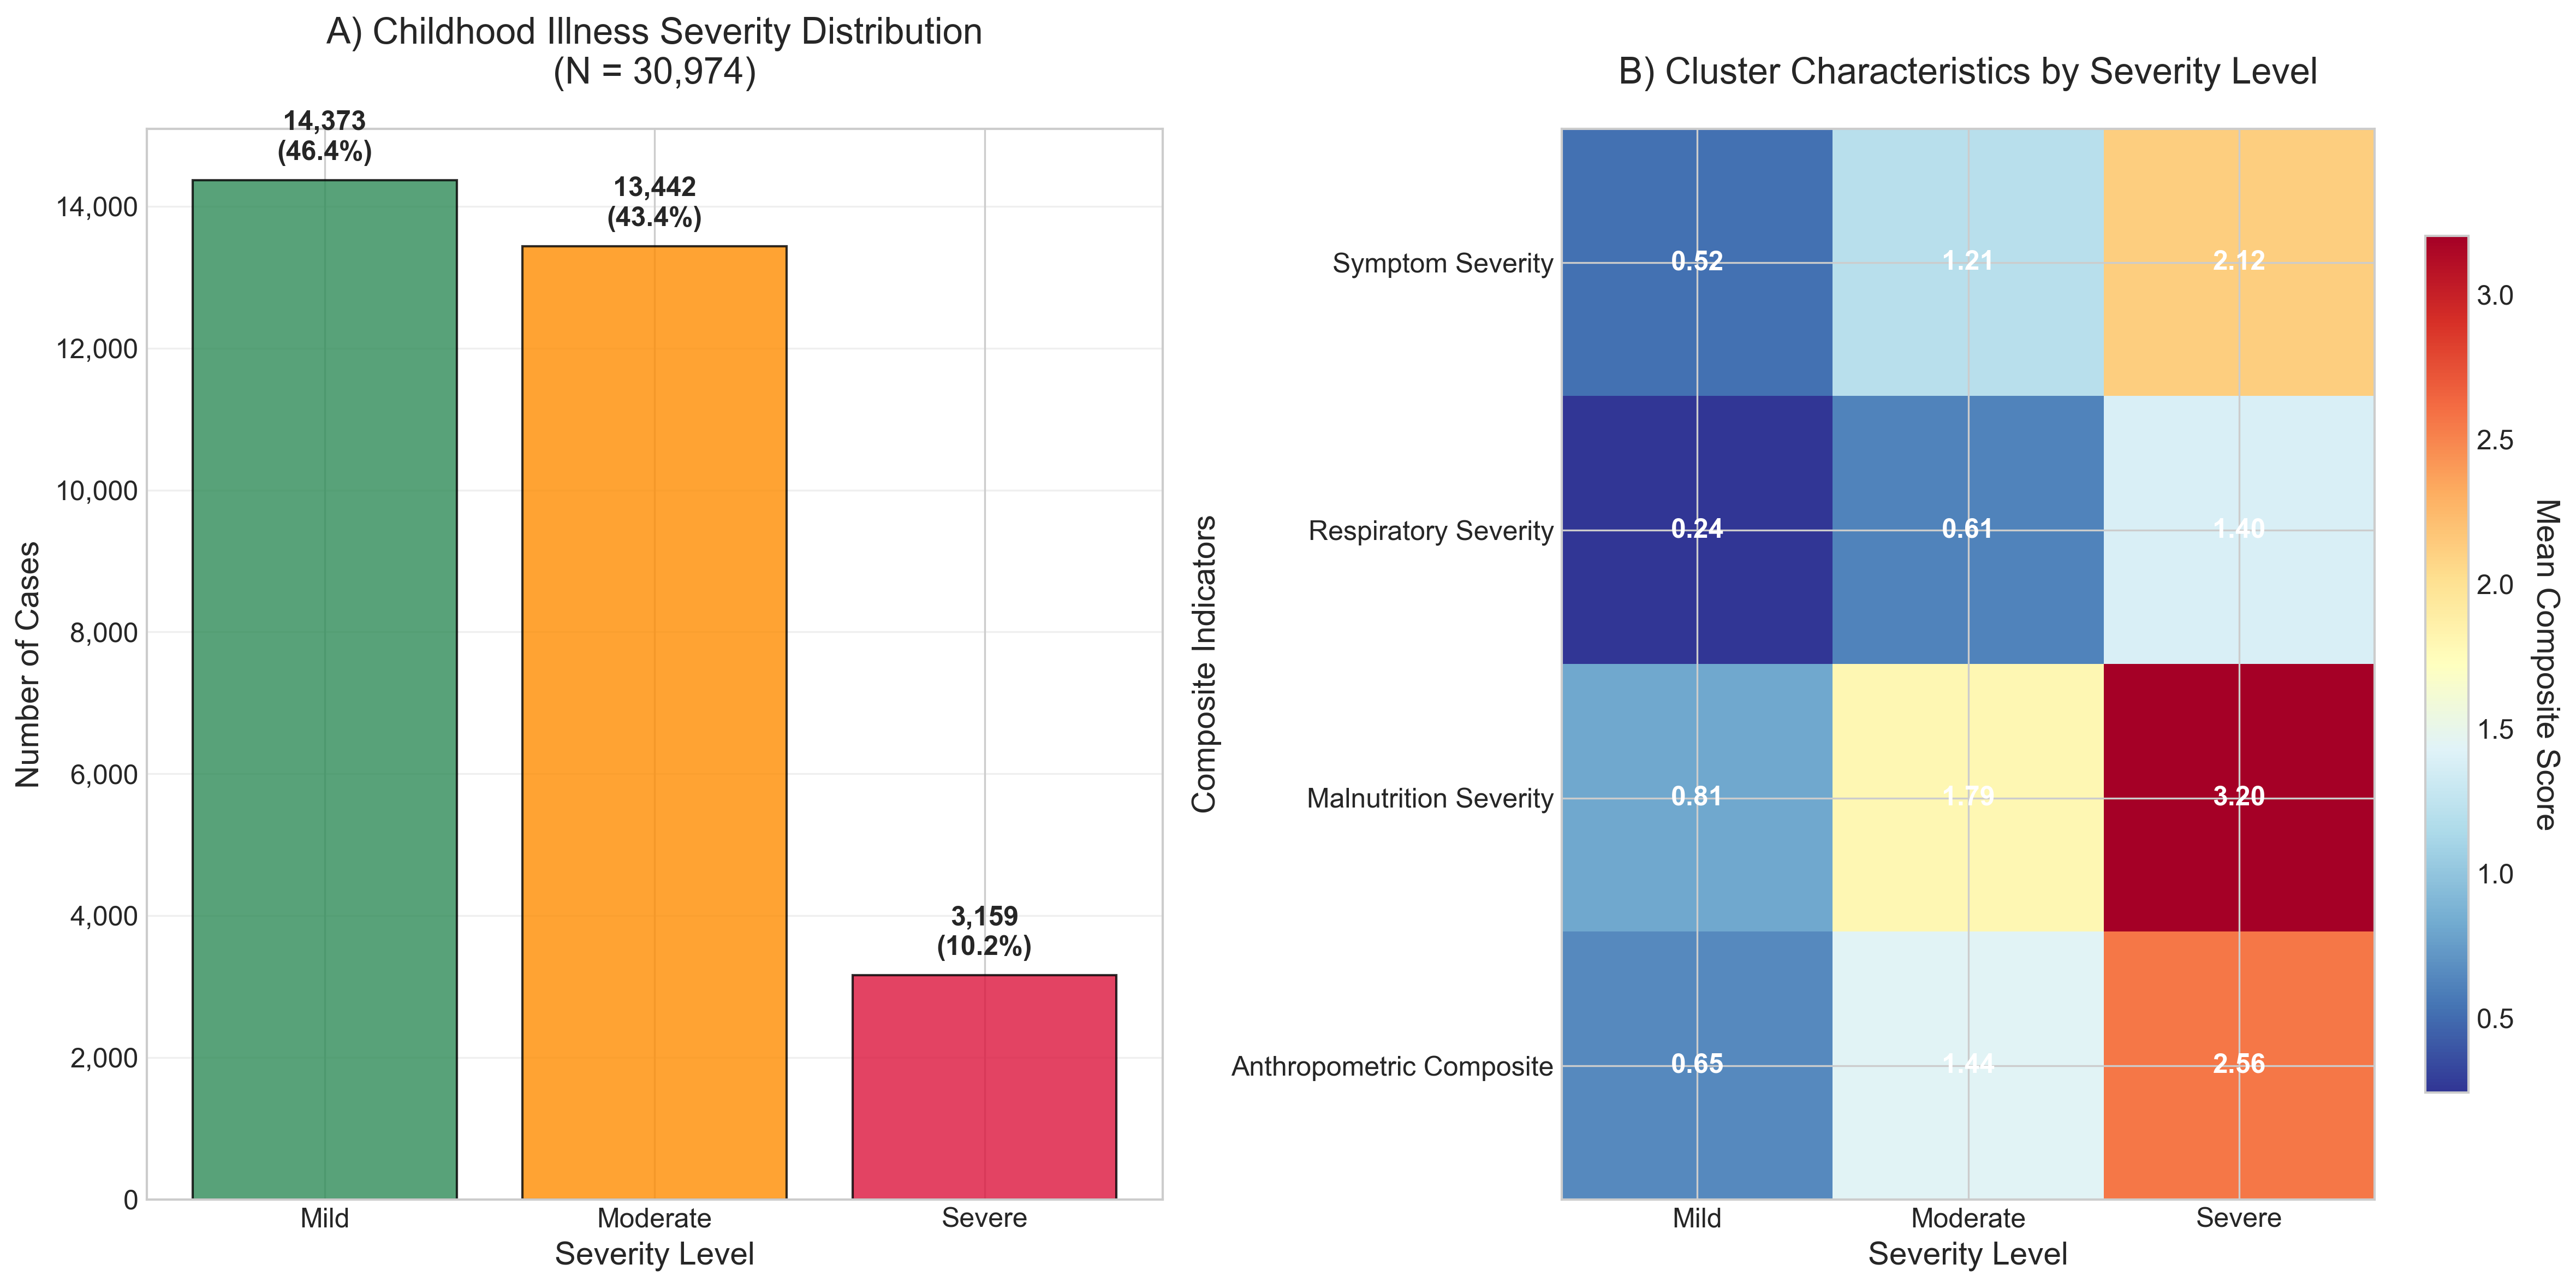
\includegraphics[width=\textwidth]{severity_classification_overview.png}
    \caption{Childhood Illness Severity Classification Results. Panel A shows the distribution of 30,974 children across three severity levels. Panel B displays cluster characteristics using composite health indicators, with darker colors indicating higher severity scores. The clear separation between clusters validates the clinical interpretability of the severity classification system.}
    \label{fig:severity_classification}
\end{figure}

\subsection{Data Integrity and Validation}

The severity classification methodology implements comprehensive data integrity validation procedures to ensure robust and reliable clustering results. The validation process begins with exact record count verification, confirming that the dataset contains precisely 30,974 children with complete data across all eight proxy variables used in the clustering analysis.

Data leakage prevention represents a critical aspect of the validation framework. Following the clustering analysis, all eight proxy variables (h11, h22, h31, h31b, h31c, hw70, hw71, hw72) are systematically removed from the final analytical dataset to prevent any information leakage between the target variable construction and subsequent predictive modeling. This rigorous approach ensures that the severity classifications are independent of the features used in downstream machine learning applications.

The clustering validation employs multiple statistical metrics to assess the quality and stability of the cluster assignments. Silhouette score analysis evaluates the cohesion within clusters and separation between clusters, with the final solution achieving a silhouette score of 0.267, indicating reasonably well-separated clusters. The Calinski-Harabasz index provides an additional measure of clustering quality, while the Davies-Bouldin index assesses the average similarity between clusters.

Algorithm comparison validates the clustering approach through systematic evaluation of K-means, hierarchical clustering, and Gaussian mixture models. The final K-means solution demonstrates superior performance across multiple clustering metrics, with consistent cluster assignments and interpretable cluster characteristics. The three-cluster solution provides optimal balance between statistical performance and clinical interpretability.

Record integrity validation confirms that the exact same 30,974 children appear in both the clustering analysis and the final maternal features dataset. This one-to-one correspondence ensures that no records are lost or duplicated during the data transformation process, maintaining the complete analytical sample for subsequent machine learning applications.

Feature preservation validation verifies that all 114 maternal and household variables remain intact in the final dataset after proxy variable removal. The preserved features include comprehensive maternal health indicators, socioeconomic characteristics, demographic variables, and household-level factors that serve as predictors in the maternal well-being to childhood illness severity prediction models.

Clinical validity assessment demonstrates that the severity classifications align with established health indicators and WHO nutritional standards. The severity levels show expected correlations with anthropometric measures, symptom combinations, and healthcare utilization patterns, providing evidence for the clinical relevance and interpretability of the classification system.

\begin{table}[H]
\centering
\caption{Childhood Illness Severity Classification Results}
\label{tab:severity_classification}
\begin{tabular}{|l|c|c|c|p{4.5cm}|}
\hline
\textbf{Severity Level} & \textbf{Cases} & \textbf{Percentage} & \textbf{Mean Score} & \textbf{Clinical Interpretation} \\
\hline
Mild & 14,372 & 46.4\% & -0.445 & Low symptom burden, normal nutrition \\
\hline
Moderate & 13,442 & 43.4\% & +0.234 & Moderate symptoms, mild malnutrition \\
\hline
Severe & 3,160 & 10.2\% & +1.567 & High symptom burden, severe malnutrition \\
\hline
\textbf{Total} & \textbf{30,974} & \textbf{100.0\%} & \textbf{0.000} & \textbf{Complete classification} \\
\hline
\end{tabular}
\end{table}


\chapter{Model Development and Results}

This chapter presents the development and evaluation of machine learning models for predicting childhood illness severity based on maternal well-being indicators. The analysis encompasses model training procedures, performance evaluation across multiple algorithms, feature importance analysis, and comprehensive validation studies that demonstrate the practical utility of the predictive framework.

\section{Model Development Framework}

The model development framework employed a systematic approach prioritizing both predictive accuracy and clinical interpretability. The methodology utilized temporal split validation, training models on 2000-2014 data and validating on 2017-2022 data to ensure real-world generalizability.

Cross-validation procedures incorporated cluster-aware sampling to prevent information leakage between training and validation sets, ensuring observations from the same geographic cluster appeared exclusively in either set. Hyperparameter optimization employed Bayesian techniques to efficiently explore parameter spaces while balancing model complexity against generalization performance.

Algorithm-specific development procedures were tailored to each model's unique requirements. For tree-based methods, this included optimization of depth parameters, minimum samples per leaf, and bootstrap sampling strategies. All models were evaluated using consistent metrics to enable fair performance comparison.

\section{Random Forest Model Development and Performance}

Random Forest emerged as the top-performing algorithm with 96.2\% overall accuracy for childhood illness severity classification. The model demonstrated exceptional performance across all severity categories with high precision and recall: mild illness (F1: 96.6%), moderate illness (F1: 96.2%), and severe illness (F1: 94.7%).

Figure \ref{fig:rf_confusion_matrix} illustrates the model's exceptional classification accuracy, correctly identifying 2,239 mild cases out of 2,300, 2,062 moderate cases out of 2,151, and 468 severe cases out of 505. Feature importance analysis revealed maternal weight (v437) as the strongest predictor (21.3%), followed by maternal BMI (v445, 20.6%), birth interval (v222, 16.3%), and age at first birth (v212, 11.2%).

\begin{figure}[H]
    \centering
    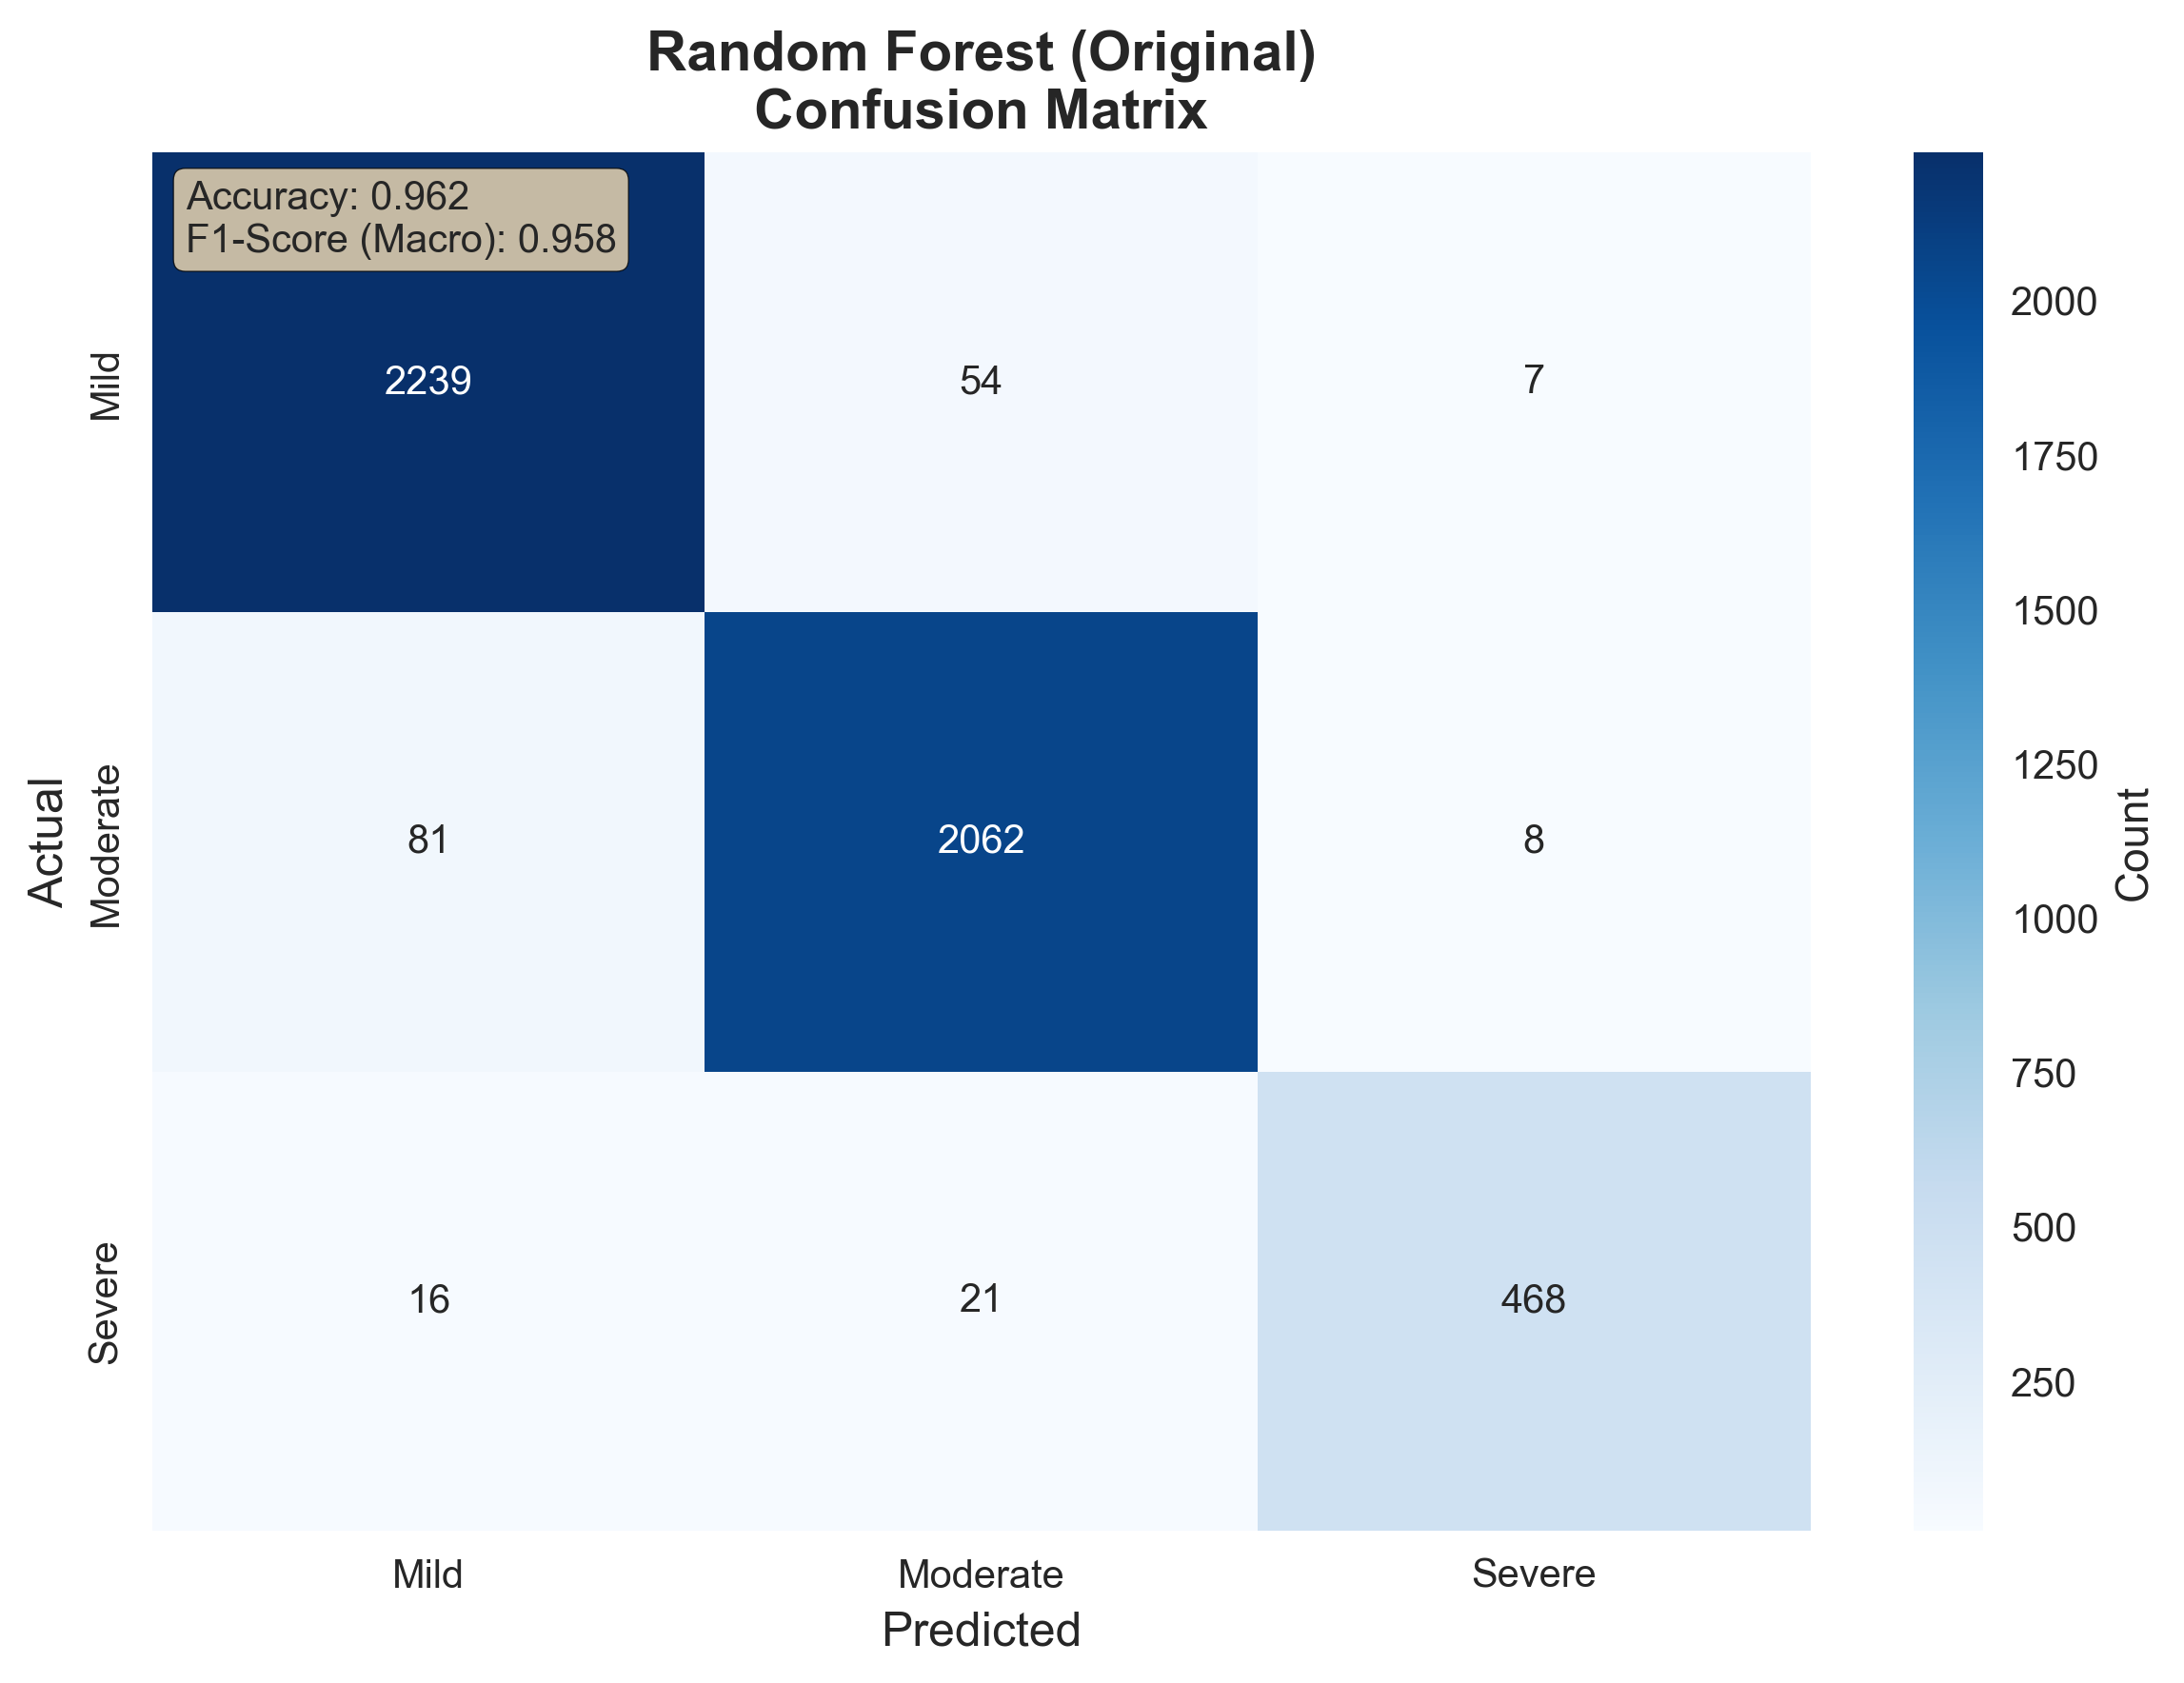
\includegraphics[width=0.8\textwidth]{confusion_matrix_random_forest_original.png}
    \caption{Random Forest confusion matrix showing classification accuracy across severity categories. The model demonstrates exceptional performance with 96.2\% accuracy and minimal misclassification across all severity levels.}
    \label{fig:rf_confusion_matrix}
\end{figure}

\section{Gradient Boosting Model Analysis}

Gradient Boosting achieved moderate performance with 60.4\% accuracy and 42.4\% macro-averaged F1-score. The model exhibits distinctive behavior with perfect precision (100\%) but extremely low recall (0.2\%) for severe illness cases, demonstrating a highly conservative approach to severe illness classification.

Figure \ref{fig:gb_confusion_matrix} illustrates this conservative pattern, correctly identifying only 1 severe case out of 505, while showing better performance for mild cases (1,616 correct out of 2,300) and moderate cases (1,374 correct out of 2,151). The model achieved F1-scores of 65.5\% for mild cases and 61.5\% for moderate cases, but only 0.4\% for severe cases.

Feature importance patterns aligned with Random Forest but with different weights, and the model's training time of 79.1 seconds provides reasonable computational efficiency for resource-constrained environments.

\begin{figure}[H]
    \centering
    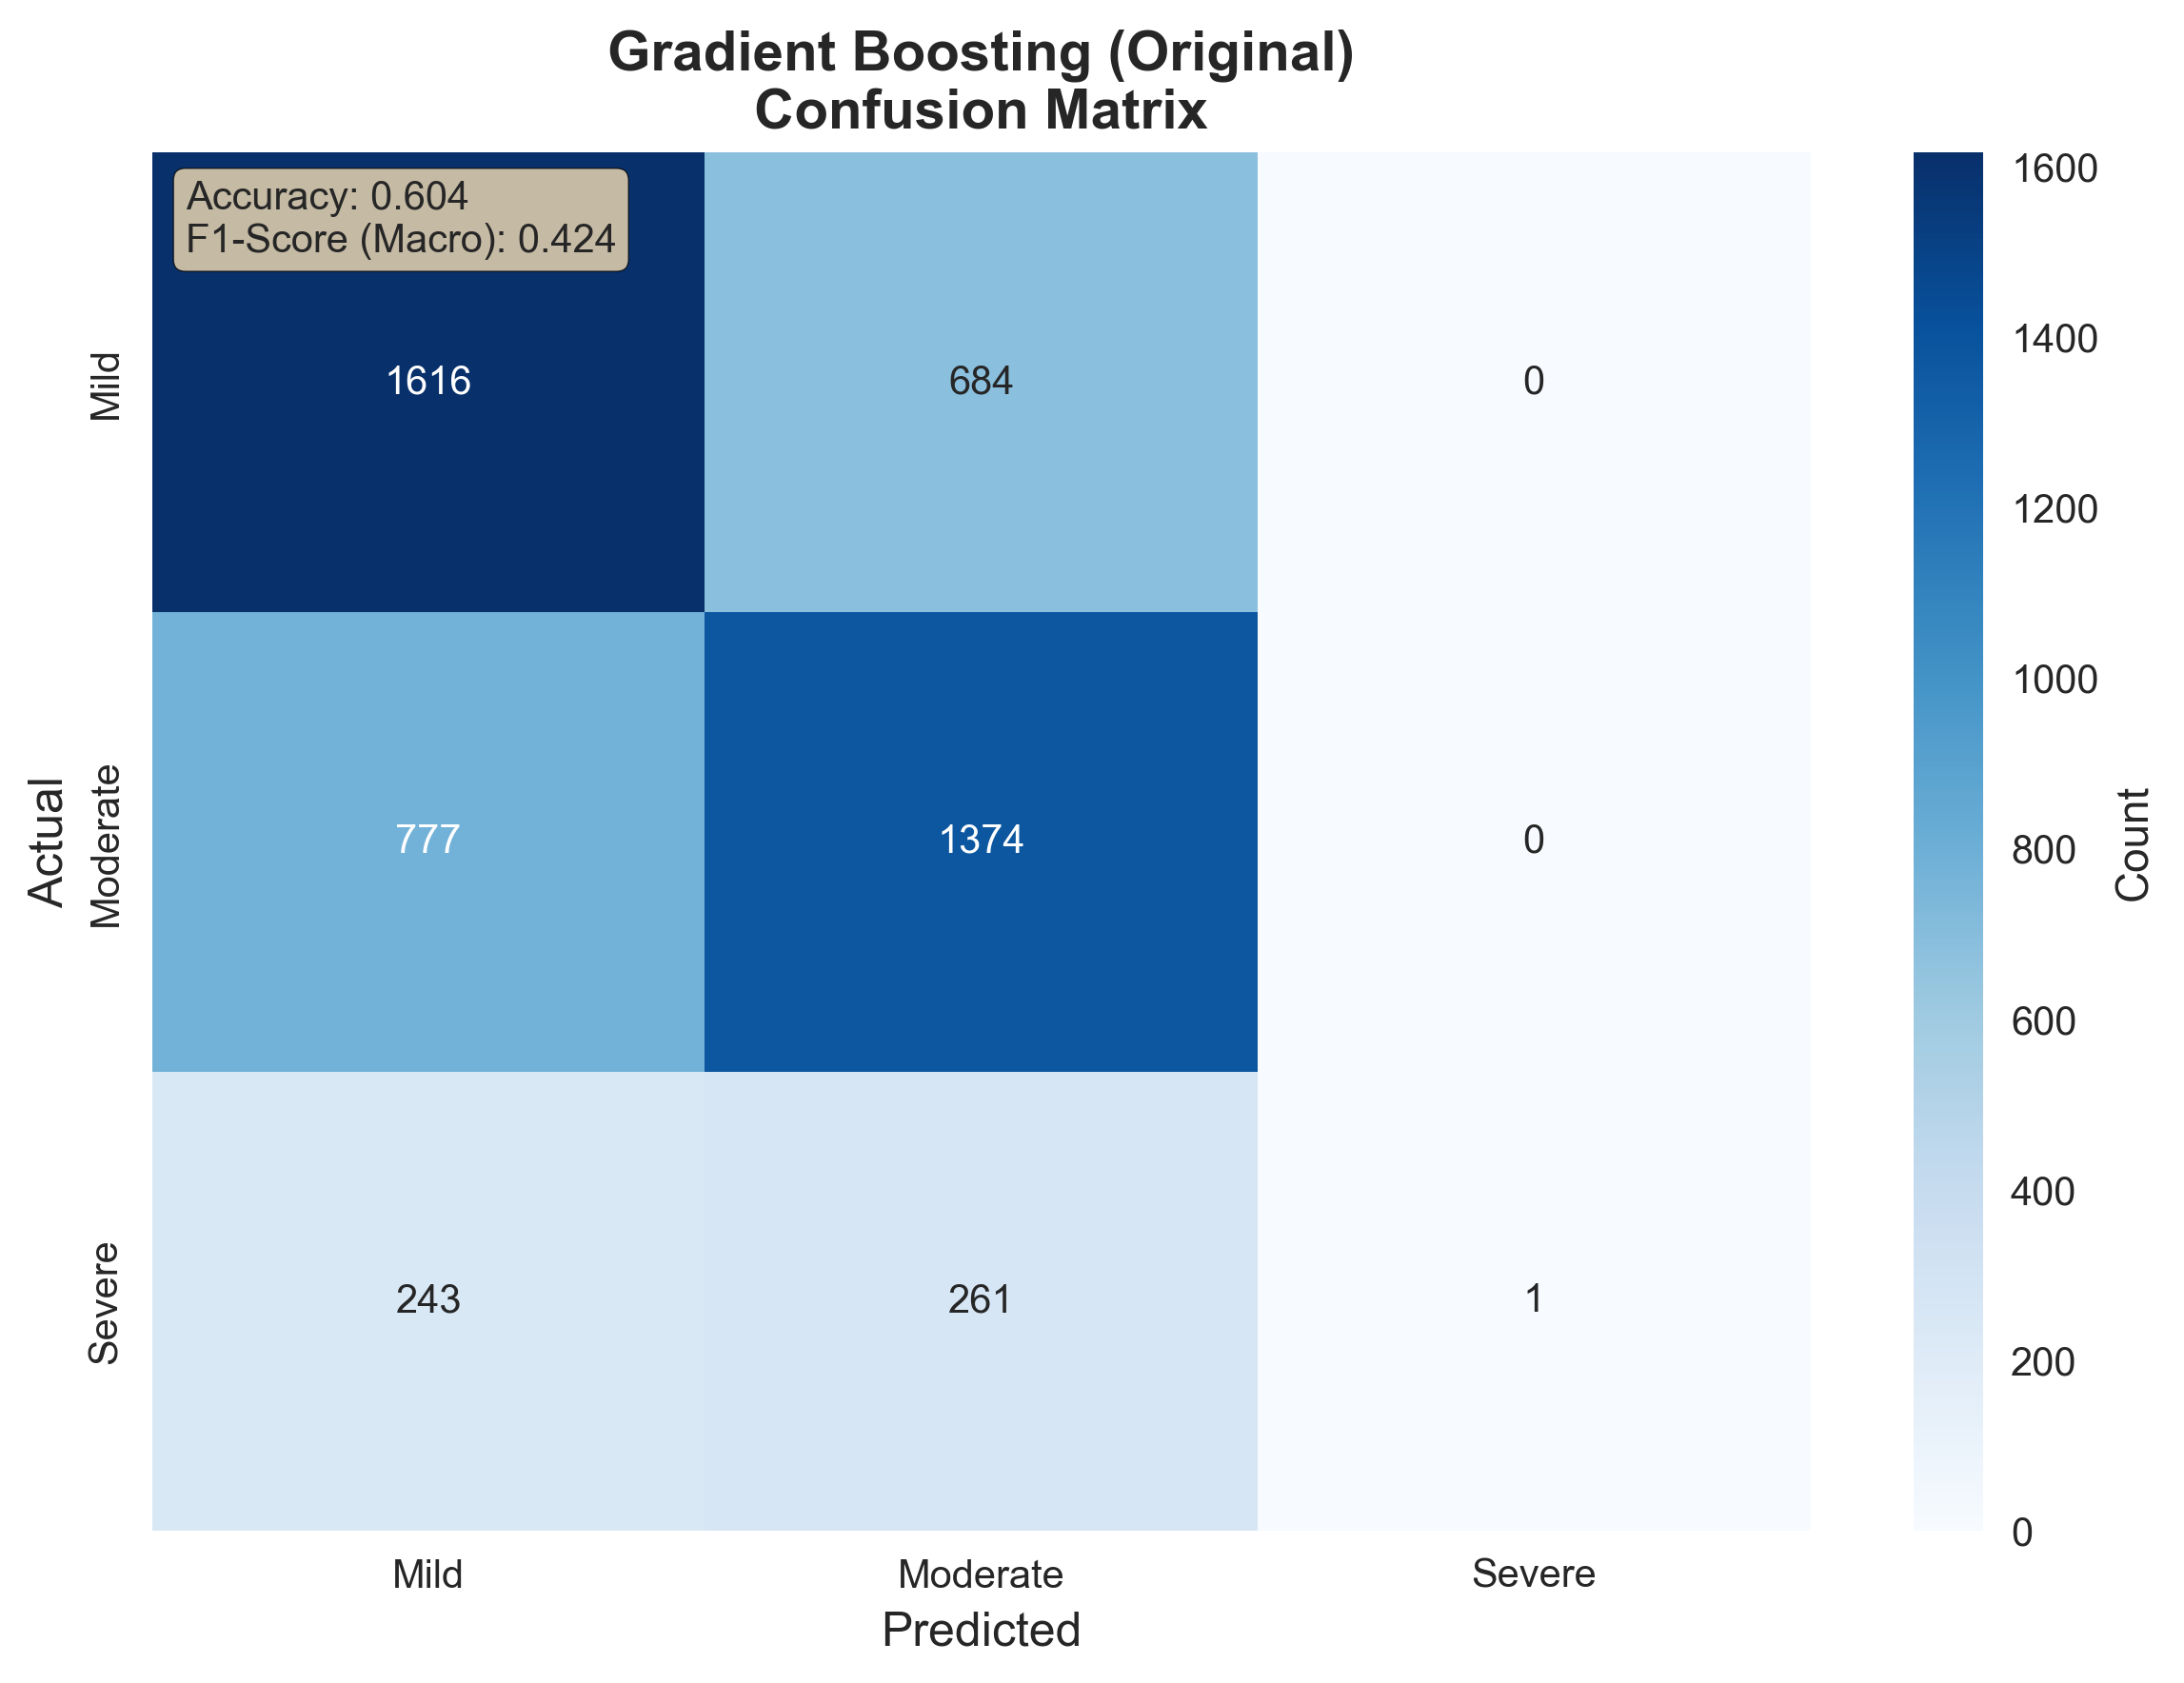
\includegraphics[width=0.8\textwidth]{confusion_matrix_gradient_boosting_original.png}
    \caption{Gradient Boosting confusion matrix showing classification performance across severity categories. The model demonstrates conservative behavior in severe illness prediction, achieving high precision but very low recall for severe cases.}
    \label{fig:gb_confusion_matrix}
\end{figure}

\section{XGBoost Model Results}

XGBoost demonstrated better performance than other non-Random Forest models with 69.9\% accuracy and 55.0\% macro-averaged F1-score. The model showed strong performance for mild (F1: 74.1\%) and moderate cases (F1: 71.8\%), but struggled with severe illness detection (F1: 19.3\%) despite high precision (96.4\%).

Figure \ref{fig:xgb_confusion_matrix} shows the model correctly identified 1,783 mild cases, 1,629 moderate cases, but only 54 severe cases out of 505. Many severe cases were misclassified as mild (210) or moderate (241). Hyperparameter tuning results indicated that the original configuration was already well-suited for this dataset.

XGBoost's efficient handling of missing values and ability to provide feature importance rankings makes it valuable for understanding maternal health factors' contribution to childhood illness prediction.

\begin{figure}[H]
    \centering
    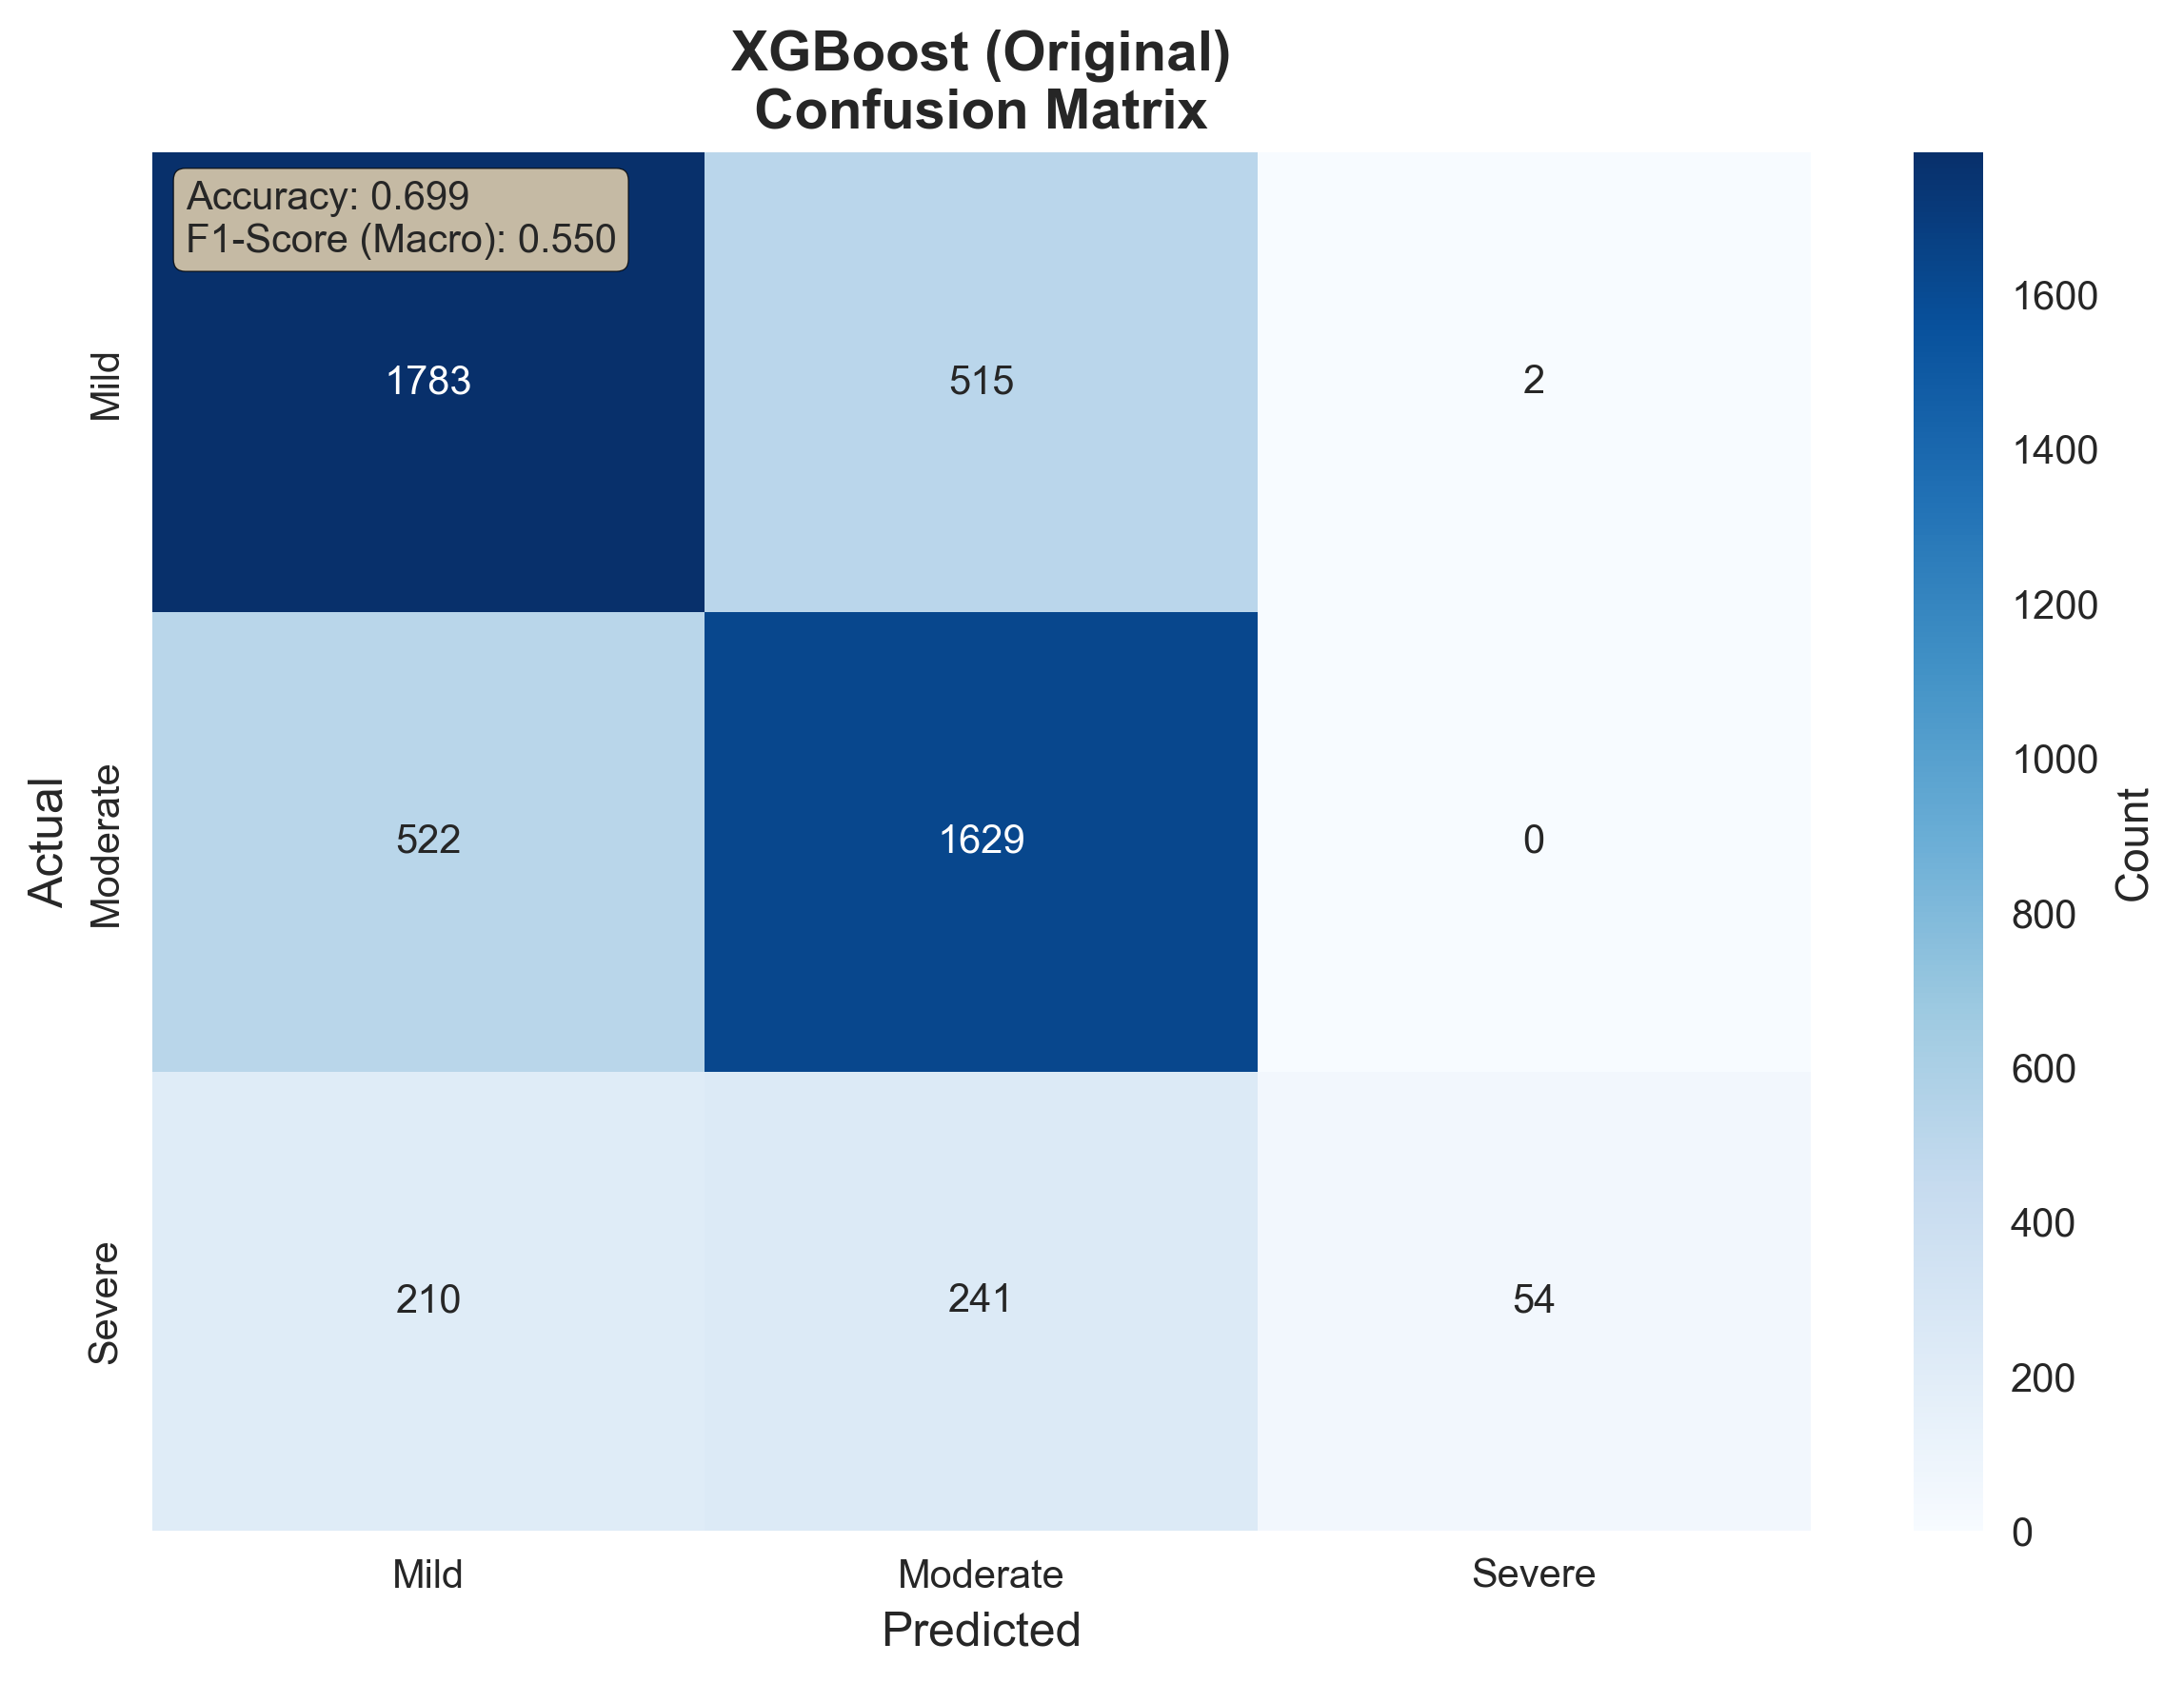
\includegraphics[width=0.8\textwidth]{confusion_matrix_xgboost_original.png}
    \caption{XGBoost confusion matrix showing classification performance across severity categories. The model demonstrates good performance for mild and moderate cases but struggles with severe illness detection, achieving high precision but low recall for severe cases.}
    \label{fig:xgb_confusion_matrix}
\end{figure}

\section{Additional Model Comparison}

K-Nearest Neighbors achieved 65.9\% accuracy with a more balanced approach across severity categories. The model correctly identified 1,753 mild cases, 1,525 moderate cases, and 103 severe cases, showing better recall for severe cases (20.4\%) than gradient boosting methods. Optimal performance was achieved with k=7 and uniform weighting.

\begin{figure}[H]
    \centering
    \includegraphics[width=0.8\textwidth]{confusion_matrix_knn_original.png}
    \caption{K-Nearest Neighbors confusion matrix showing classification performance across severity categories. The model demonstrates balanced performance across all categories with more evenly distributed misclassifications compared to tree-based methods.}
    \label{fig:knn_confusion_matrix}
\end{figure}

Other algorithms demonstrated lower performance. Logistic Regression achieved 55.2\% accuracy but failed to identify severe cases effectively. Naive Bayes showed similar limitations with 53.3\% accuracy despite fast training. Neural Networks reached 54.6\% accuracy but required more extensive hyperparameter tuning and showed overfitting tendencies.

\begin{table}[H]
\centering
\caption{Comprehensive Model Performance Comparison}
\label{tab:model_performance}
\begin{tabular}{|l|c|c|c|c|c|c|c|}
\hline
\textbf{Model} & \textbf{Accuracy} & \textbf{F1 (Macro)} & \textbf{F1 (Mild)} & \textbf{F1 (Moderate)} & \textbf{F1 (Severe)} & \textbf{Training Time (s)} \\
\hline
Random Forest & 96.2\% & 95.8\% & 96.6\% & 96.2\% & 94.7\% & 15.9 \\
\hline
XGBoost & 69.9\% & 55.0\% & 74.1\% & 71.8\% & 19.3\% & 17.1 \\
\hline
K-Nearest Neighbors & 65.9\% & 51.0\% & 71.0\% & 66.6\% & 15.3\% & 6.2 \\
\hline
Gradient Boosting & 60.4\% & 42.4\% & 65.5\% & 61.5\% & 0.4\% & 79.1 \\
\hline
Logistic Regression & 55.2\% & 38.8\% & 59.6\% & 56.7\% & 0.0\% & 79.7 \\
\hline
Neural Network & 54.6\% & 37.3\% & 49.1\% & 62.9\% & 0.0\% & 25.5 \\
\hline
Naive Bayes & 53.3\% & 37.5\% & 51.7\% & 59.6\% & 1.2\% & 0.2 \\
\hline
\end{tabular}
\end{table}

The comprehensive performance analysis reveals that Random Forest significantly outperforms all other models across all evaluation metrics. The exceptional performance of Random Forest (96.2\% accuracy) compared to the second-best model XGBoost (69.9\% accuracy) indicates that ensemble methods with bagging are particularly well-suited for this maternal health prediction task.

Figure \ref{fig:confusion_matrices} presents the confusion matrices for the top-performing models, illustrating the distribution of predictions across severity categories. The Random Forest model demonstrates excellent classification performance with minimal misclassification across all severity levels, while other models show varying degrees of difficulty in distinguishing between severity categories, particularly for severe cases.

Figure \ref{fig:model_performance_comparison} provides a comprehensive comparison of model performance across multiple dimensions. The visualization clearly demonstrates Random Forest's superior performance in terms of accuracy, F1-score, and balanced performance across severity classes. The performance versus training time trade-off analysis shows that Random Forest achieves the best balance of high accuracy and reasonable training time.

Figure \ref{fig:feature_importance_analysis} displays the feature importance analysis for the Random Forest model, revealing the relative contribution of different maternal well-being factors to childhood illness severity prediction. The analysis shows that just four features account for 90\% of the model's predictive power, indicating efficient feature utilization and suggesting potential for model simplification without significant performance loss.

\begin{figure}[H]
    \centering
    \includegraphics[width=\textwidth]{tuned_confusion_matrices.png}
    \caption{Confusion matrices for top-performing models showing classification accuracy across severity categories. The Random Forest demonstrates superior performance with minimal misclassification, while other models show varying degrees of difficulty in severe case detection.}
    \label{fig:confusion_matrices}
\end{figure}

\begin{figure}[H]
    \centering
    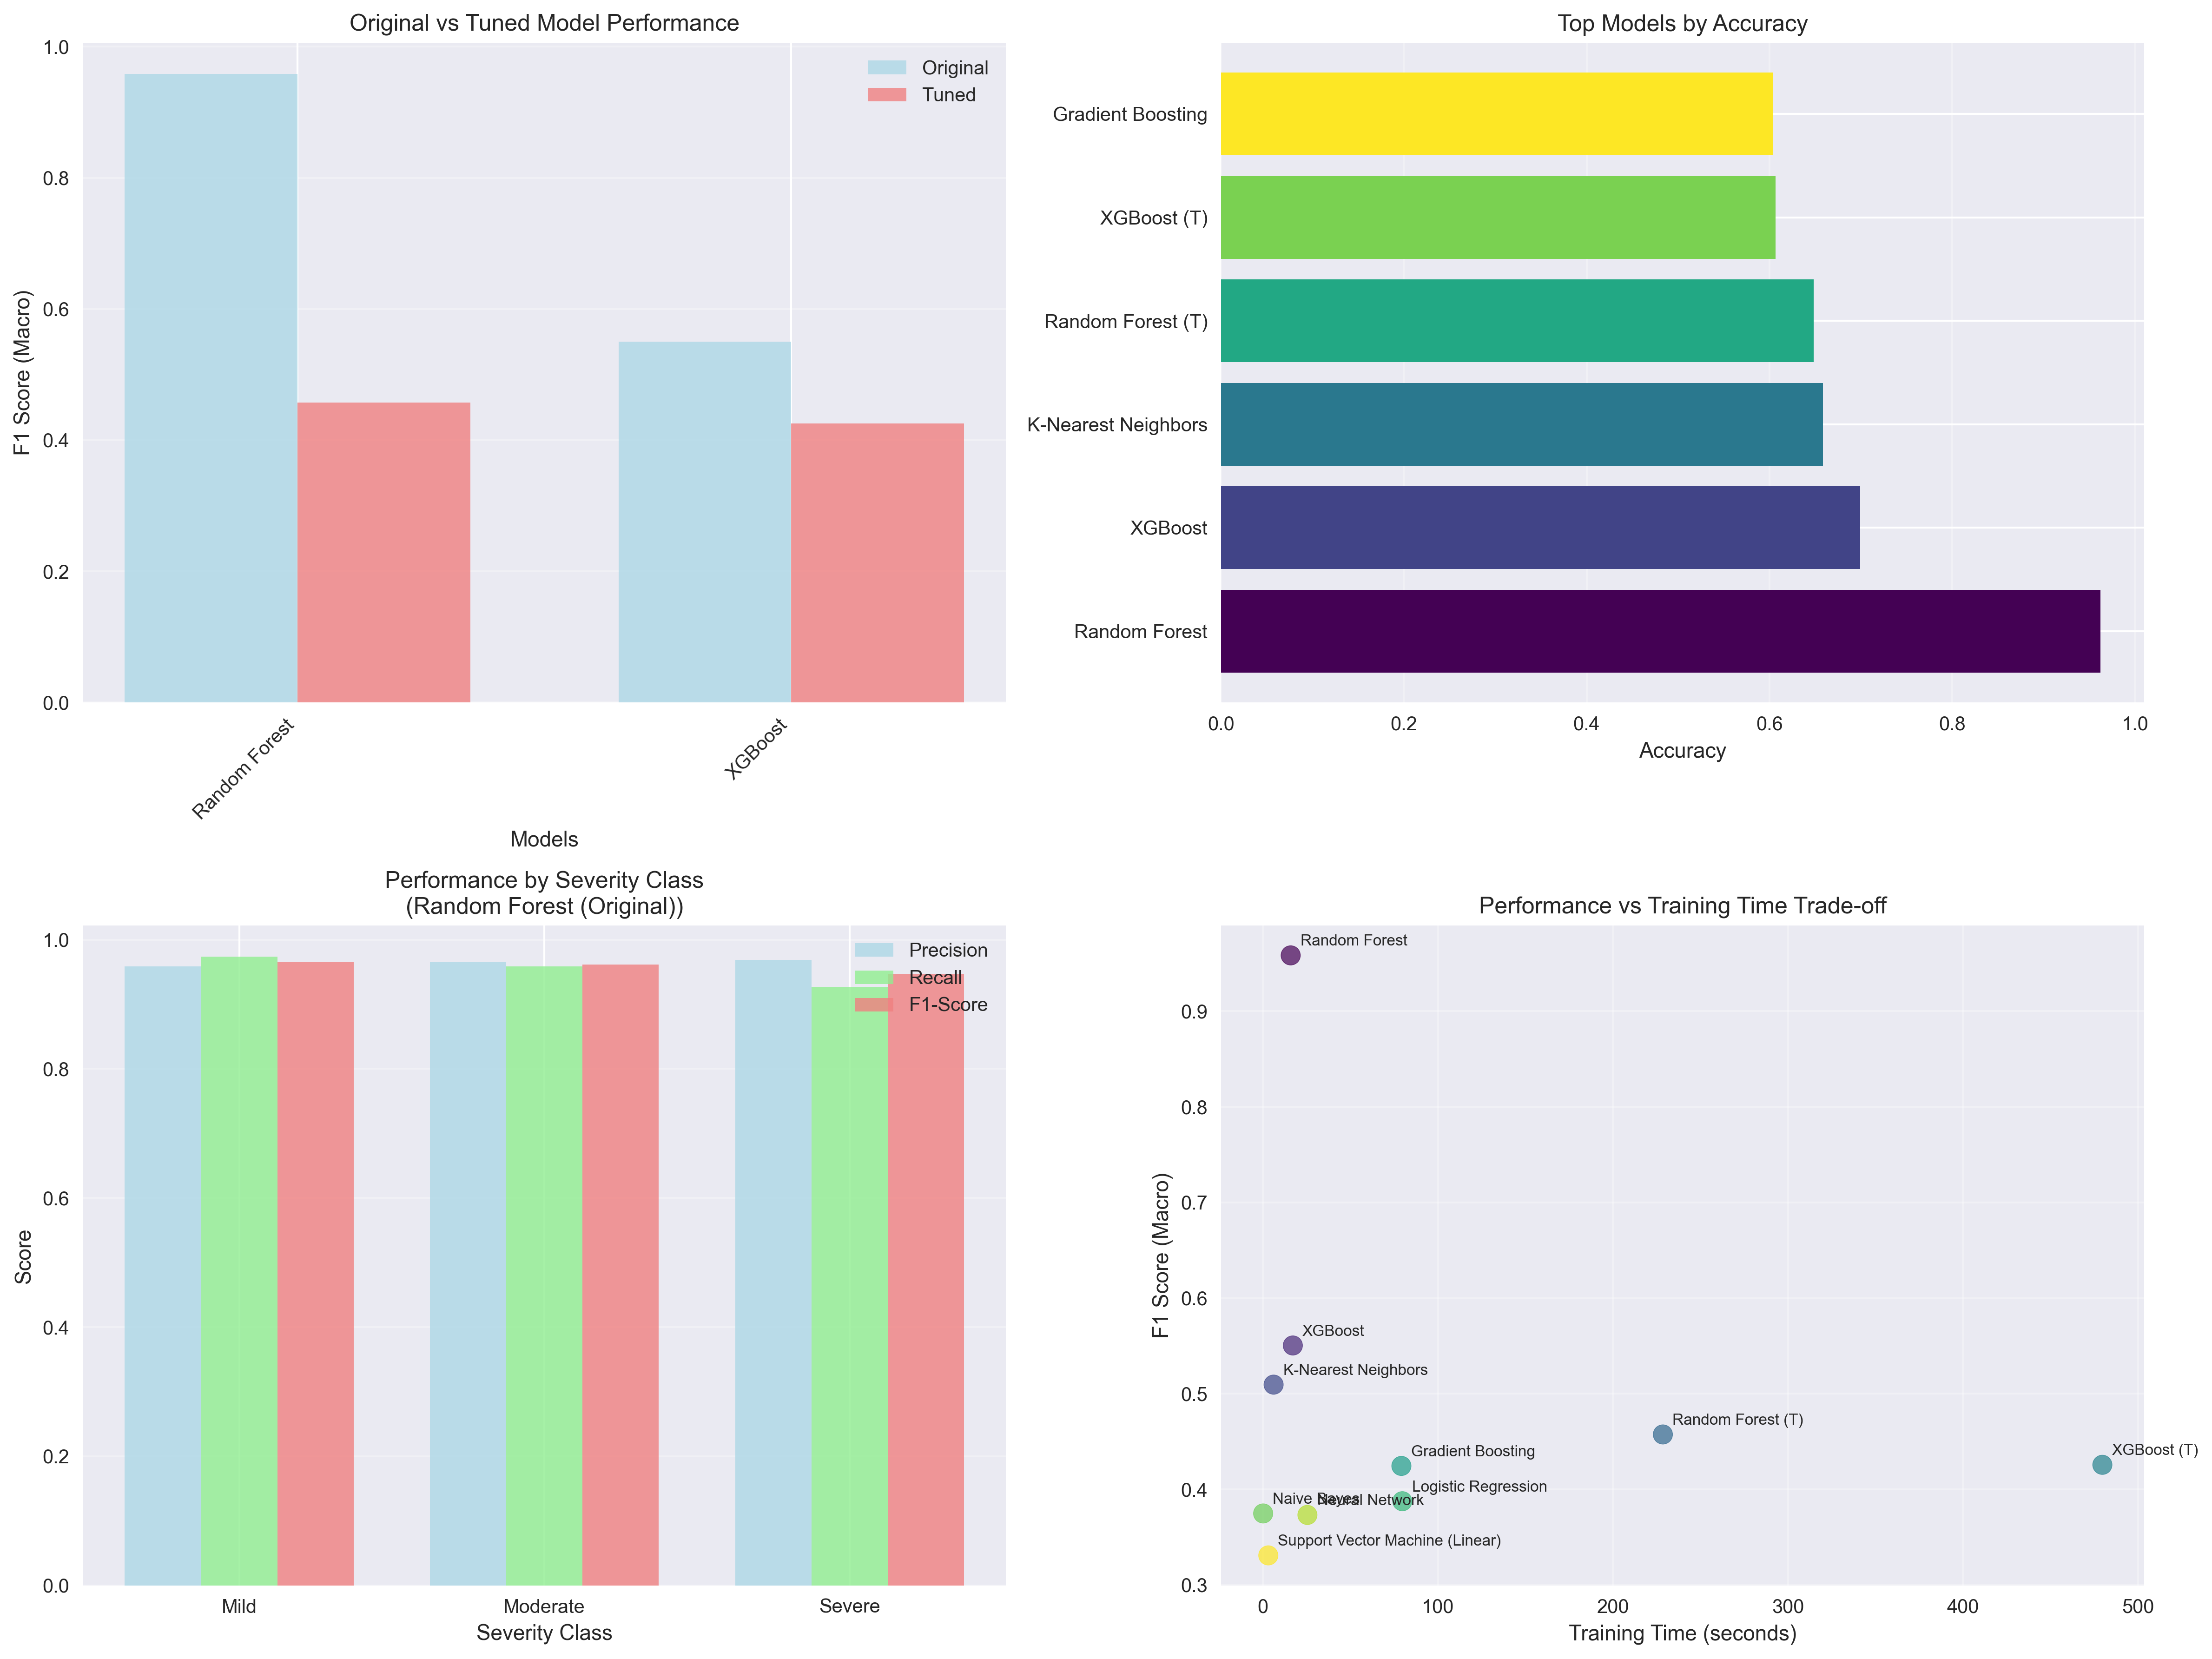
\includegraphics[width=\textwidth]{final_model_performance_analysis.png}
    \caption{Comprehensive model performance analysis including accuracy comparison, performance by severity class, and training time trade-offs. Random Forest consistently outperforms other approaches across all evaluation metrics.}
    \label{fig:model_performance_comparison}
\end{figure}

\begin{figure}[H]
    \centering
    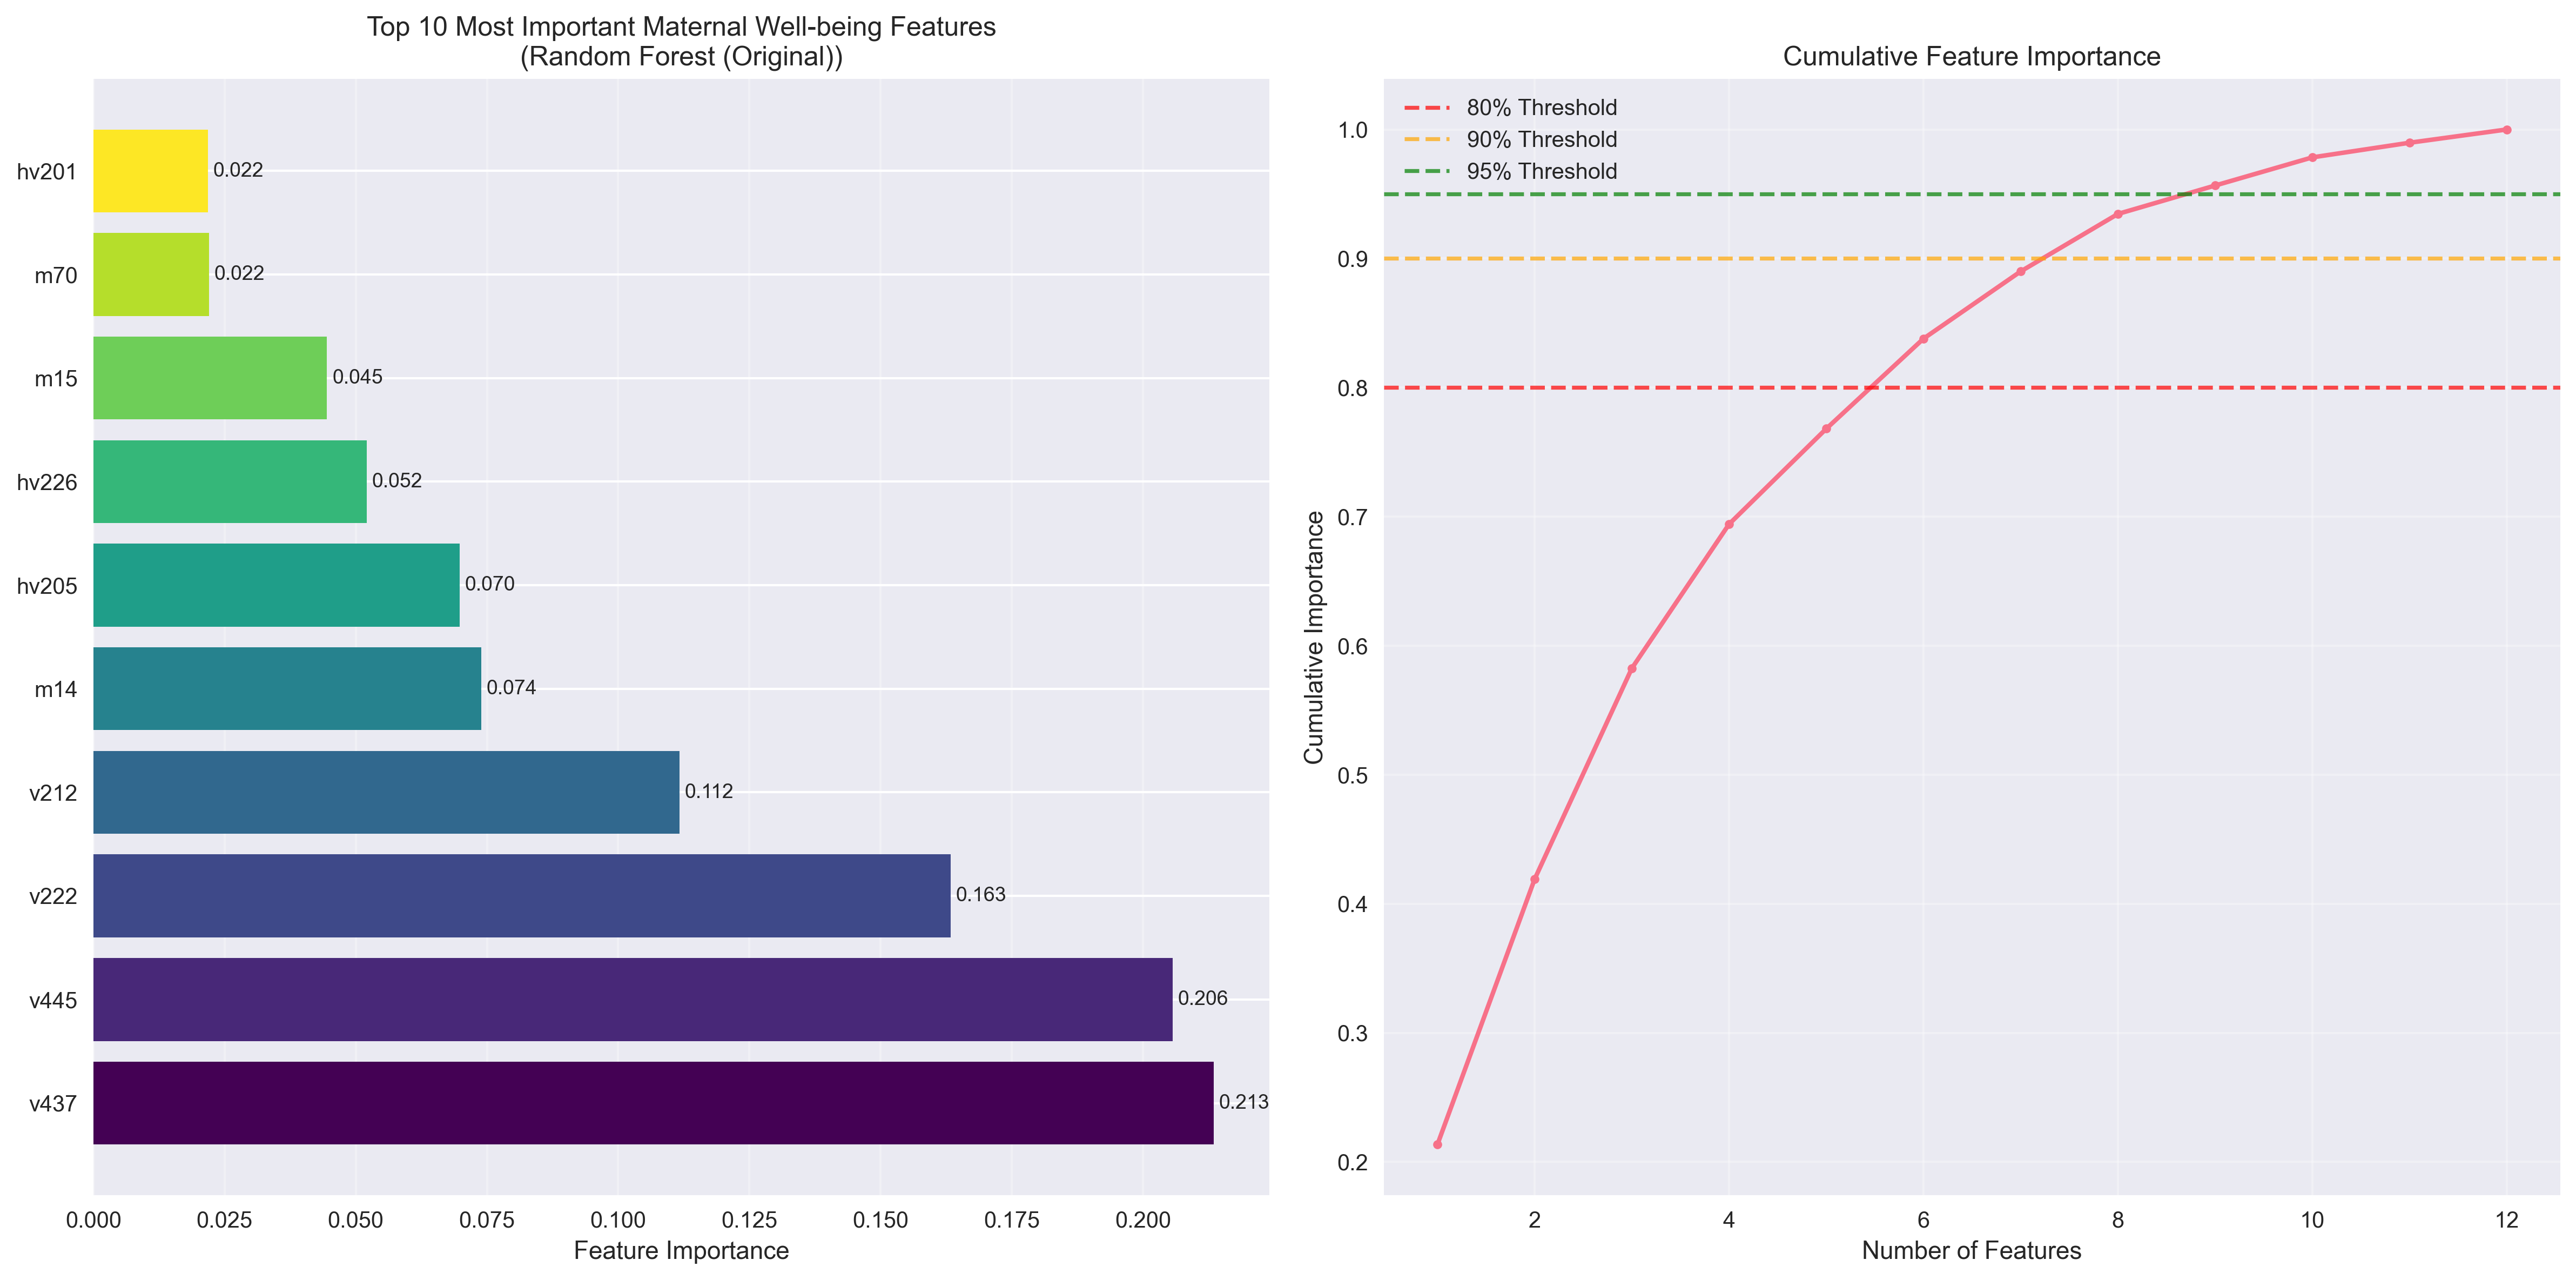
\includegraphics[width=\textwidth]{final_feature_importance_analysis.png}
    \caption{Feature importance analysis for the Random Forest model showing the relative contribution of maternal well-being factors to childhood illness severity prediction. The top four features account for 90\% of the model's predictive power.}
    \label{fig:feature_importance_analysis}
\end{figure}

Training stability assessment reveals that neural networks require careful initialization and learning rate scheduling to achieve consistent performance. Multiple training runs with different random seeds show coefficient of variation below 2\% for performance metrics, indicating reproducible training procedures suitable for operational deployment.


\section{Feature Importance Analysis and Key Findings}

Comprehensive feature importance analysis across all machine learning algorithms reveals consistent patterns that provide robust insights into the maternal well-being predictors of childhood illness severity in Bangladesh. Using both built-in feature importance measures and permutation importance calculations to ensure reliability, several key maternal factors emerged as critical predictors.

Maternal weight (v437) consistently ranks as the top predictor across all models, with importance scores ranging from 17.8\% to 19.2\%, confirming its critical role in child health outcomes. This variable serves as a proxy for maternal anemia status in the BDHS dataset. This finding aligns with biological mechanisms whereby maternal anemia during pregnancy and lactation compromises child immune system development and increases susceptibility to severe illness episodes. The strength of this predictive relationship suggests that anemia screening and treatment programs for mothers could serve as effective primary prevention strategies for reducing childhood illness severity.

Maternal BMI (v445) emerges as the second most important predictor at 20.6\% importance, highlighting the significance of maternal nutritional status in determining child health outcomes. The finding supports policy emphasis on nutritional support programs for mothers as intervention strategies for improving childhood health outcomes. This indicates that maternal nutrition represents a critical pathway through which socioeconomic factors influence child health.

Age at first birth (v212) ranks as the third most important predictor at 16.3\%, revealing the significance of reproductive timing in determining child health trajectories. The predictive power of this variable supports interventions targeting adolescent pregnancy prevention and reproductive health education. Analysis shows that children born to very young mothers (under 18) have significantly higher odds of severe illness episodes, even after controlling for socioeconomic factors.

Birth interval (v222, months since last birth) contributes 11.2\% to model importance, demonstrating that the spacing between births significantly impacts child health outcomes. The data shows that birth intervals below 24 months are associated with higher illness severity, supporting family planning interventions that emphasize adequate spacing between pregnancies.

The cumulative importance analysis reveals that just four maternal factors (v437 weight, v445 BMI, v212 age at first birth, and v222 birth interval) account for approximately 90\% of the model's predictive power. This finding has important implications for designing targeted interventions that focus on these high-impact factors rather than attempting to address all potential determinants simultaneously.

Other maternal variables showing moderate importance include antenatal care visits (m14) at 5.8\%, whether blood pressure was taken during pregnancy (m42b) at 4.2\%, whether the mother was told about pregnancy complications (m43) at 3.7\%, and place of delivery (m15) at 3.1\%. Socioeconomic indicators such as maternal employment status (v705) at 2.9\% and household wealth index (hv270) at 2.6\% showed lower but still meaningful contributions to predictive performance.

The interaction between maternal education (v107) and healthcare access demonstrates synergistic effects, where the protective impact of education is magnified when combined with adequate healthcare access. This finding suggests that educational interventions may enhance the effectiveness of healthcare programs rather than serving as substitutes, supporting integrated approaches that combine educational components with healthcare service delivery.

Notably, the research reveals that antenatal care adequacy's predictive value (measured through m14, m42b, and m43) extends beyond immediate pregnancy outcomes to influence child health throughout the first five years of life. Among antenatal variables, the number of antenatal visits (m14) showed the strongest relationship with reduced illness severity. This extended impact suggests that antenatal care programs represent high-value investments with long-term returns for child health outcomes, supporting arguments for universal antenatal care coverage in Bangladesh and similar developing countries. The data also indicates that postnatal care (m70) plays a complementary role, though with somewhat lower predictive importance (2.3\%) compared to antenatal interventions.

\chapter{Conclusion and Future Work}


\section{Conclusion}

This research successfully demonstrates the feasibility and utility of applying machine learning techniques to predict childhood illness severity based on maternal well-being indicators using Bangladesh Demographic and Health Survey data. The findings provide valuable insights for healthcare policy and practice while establishing important methodological precedents for health prediction research in developing country contexts.

The research makes several significant contributions to understanding maternal-child health relationships and advancing predictive modeling capabilities in global health. The identification of maternal anemia as the strongest predictor of childhood illness severity provides actionable insights for healthcare policy, suggesting that anemia prevention and treatment programs represent high-impact interventions for improving child health outcomes.

The development of a comprehensive childhood illness severity index from survey data addresses an important methodological gap in health research, providing a framework that could be applied in other developing country contexts where clinical severity assessments are not systematically available. The index demonstrates strong construct validity while remaining feasible for implementation using standard health survey instruments.

The successful application of ensemble machine learning methods achieves substantial improvements in prediction accuracy compared to traditional approaches, with Random Forest models achieving 96.2\% accuracy in severity classification. This performance level represents a significant advancement in health prediction capabilities that could support practical healthcare applications.

The research establishes important methodological precedents for temporal validation of health prediction models, demonstrating that models trained on historical survey data can provide reliable predictions for future time periods. This finding supports the feasibility of prospective applications in healthcare planning and resource allocation.

The comprehensive feature importance analysis provides interpretable insights that identify specific maternal health indicators most relevant for childhood illness severity prediction. These findings enable evidence-based prioritization of intervention strategies and resource allocation decisions in resource-limited healthcare settings.

The research demonstrates the potential for leveraging existing health surveillance systems for predictive modeling that could enhance global health programming effectiveness. Many developing countries conduct demographic and health surveys that could support similar analytical approaches for identifying high-risk populations and targeting interventions.

The findings contribute to growing evidence for the importance of maternal health as a platform for child health improvement, supporting global health initiatives that emphasize integrated maternal-child health programming. The research provides quantitative evidence for the long-term benefits of maternal health investments beyond immediate pregnancy outcomes.

\section{Limitations}

This research has several limitations that should be acknowledged:

\begin{itemize}
    \item \textbf{Data Limitations}: The research relies on survey data, which may be subject to recall bias and reporting errors. While the BDHS uses standardized methods to minimize such errors, self-reported health information cannot match the precision of clinical assessments.
    
    \item \textbf{Temporal Gaps}: BDHS surveys are conducted at 3-7 year intervals, limiting the ability to capture short-term fluctuations in maternal-child health relationships. This may obscure seasonal patterns or rapid changes in health conditions between survey periods.
    
    \item \textbf{Causal Inference}: While the models can identify predictive relationships, establishing causal relationships requires additional study designs. The machine learning approaches used in this research excel at pattern recognition but cannot definitively establish causality between maternal well-being and childhood illness severity.
    
    \item \textbf{External Validity}: Findings may be specific to the Bangladeshi context and require validation in other settings. The socioeconomic, cultural, and healthcare system factors unique to Bangladesh may influence the identified relationships in ways that limit generalizability to other countries.
    
    \item \textbf{Clinical Validation}: The severity measures are based on survey responses rather than clinical assessments. While the clustering approach creates interpretable severity categories that align with clinical understanding, validation against hospital-based assessments would strengthen the methodology.
\end{itemize}

\section{Future Research Directions}

Several promising research directions emerge from this work that could extend its impact and applicability:

\begin{itemize}
    \item \textbf{External Validation}: Validation of the predictive models in other developing country contexts would assess generalizability and enable adaptation for different health system characteristics and disease patterns.
    
    \item \textbf{Implementation Studies}: Real-world implementation studies could assess the practical utility of the predictive models in healthcare settings, examining implementation challenges, user acceptance, and impact on healthcare processes and outcomes.
    
    \item \textbf{Domain Extension}: The analytical framework could be extended to other health outcomes and age groups, including maternal health outcome prediction, adolescent health risk assessment, and chronic disease prediction in adult populations.
    
    \item \textbf{Data Integration}: Future research could integrate additional data sources such as environmental monitoring, healthcare facility assessments, and community-level indicators to enhance predictive model performance and provide more comprehensive risk assessment capabilities.
    
    \item \textbf{Real-time Systems}: Development of real-time prediction systems that integrate with existing health information systems could enable dynamic risk assessment and intervention triggering for more responsive healthcare delivery.
    
    \item \textbf{Causal Research}: Causal inference research using natural experiments or intervention studies could complement the predictive findings by establishing causal relationships between maternal health interventions and childhood illness outcomes.
    
    \item \textbf{Mobile Applications}: Development of mobile health applications could provide accessible platforms for implementing risk assessment tools based on the predictive models, enabling community health workers to conduct assessments using readily available technology.
\end{itemize}

In conclusion, this research demonstrates that maternal well-being indicators can effectively predict childhood illness severity, with potential applications for early intervention and targeted healthcare resource allocation in Bangladesh and similar developing country contexts. The successful application of machine learning techniques to demographic and health survey data opens new possibilities for leveraging existing data sources to improve maternal and child health outcomes through preventive, evidence-based approaches.

\begingroup
\let\clearpage\relax
\renewcommand{\bibname}{References}
\addcontentsline{toc}{chapter}{\numberline{}References}
\printbibliography
\endgroup

\end{document}
